To measure the efficiency of the \Pgg-specific component of the photon ID, we use a \sieie\ template fit to extract the number of true photons from a pool of photon objects passing the \egamma\ ID.

The measurement is performed using the EM object+jet measurement sample. 
We fit the \sieie\ distribution of the EM object with a template describing the \sieie\ shape of true photons and another describing the hadronic background. 
The real photon template is taken from \gj\ MC requiring the photon to pass the \egamma\ ID except for the \sieie\ requirement.
The fake photon template is taken from the same data control sample, requiring $5\GeV < \ICH < 7\GeV$.
The number of true photons in the target sample is the integral of the post-fit real photon template below $\sieie = 0.0104$, the same value as in our photon ID. 

The fit is performed once for all EM objects and then once for EM objects passing the \Pgg-specific ID criteria. 
The ratio of the numbers of true photons obtained in the two fits is the efficiency.

The \sieie\ template fit method in its simplest form fits the observed distribution with the following fit function:
\begin{align}
  P(f;\sieie) = f \cdot h_{s}(\sieie) + (1 - f) \times h_{b}(\sieie),
\end{align}
where $h_{s}$ is the signal template, $h_{b}$ is the background template, and $f$ is the fraction of true photons in the target sample. 
Both the target template and the fit function are normalized to unity, removing the number of photon candidates in the target sample $N$ as a fit parameter and leaving $f$ as the only free parameter.

\begin{figure}[htbp]
  \centering
  \resizebox{\textwidth}{!}{
    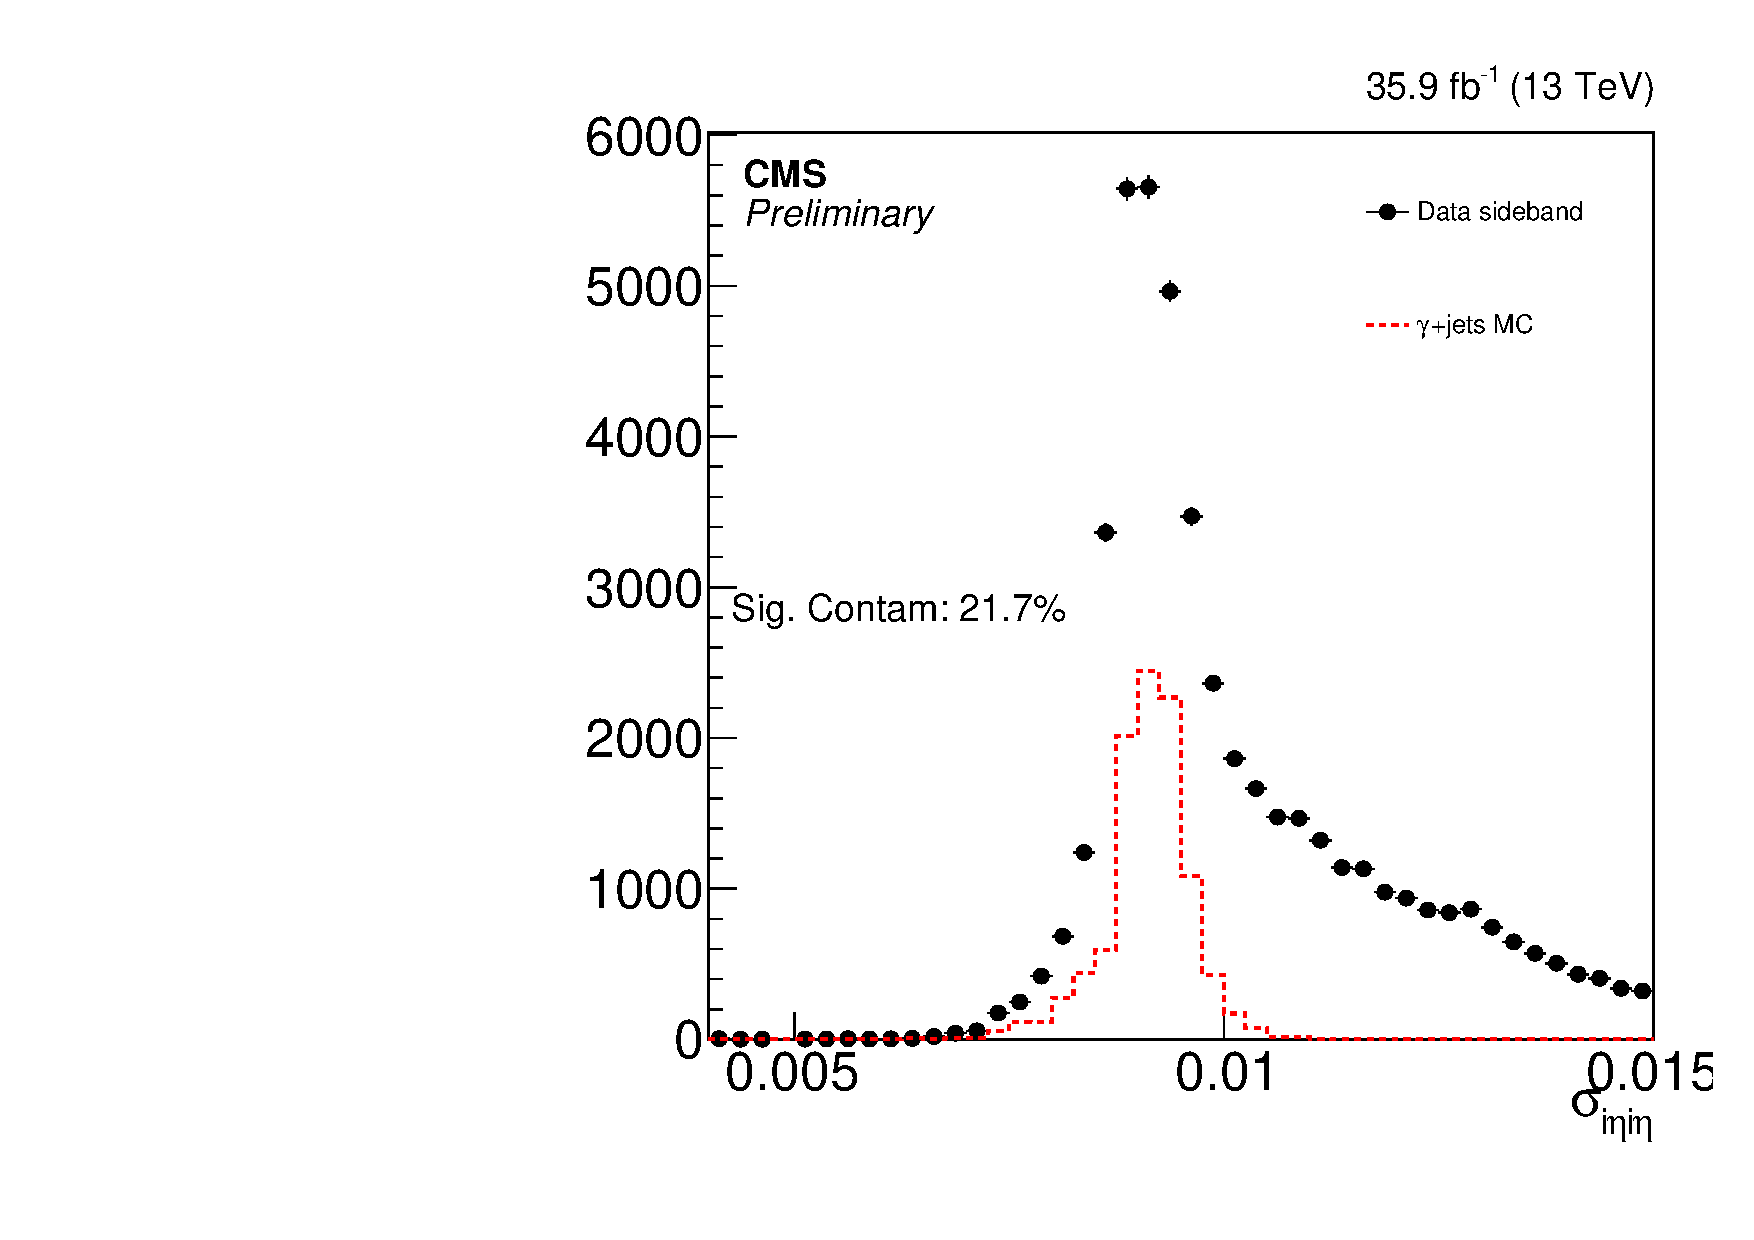
\includegraphics[]{Analysis/Figures/pvsf/sbcontam_near.pdf}
    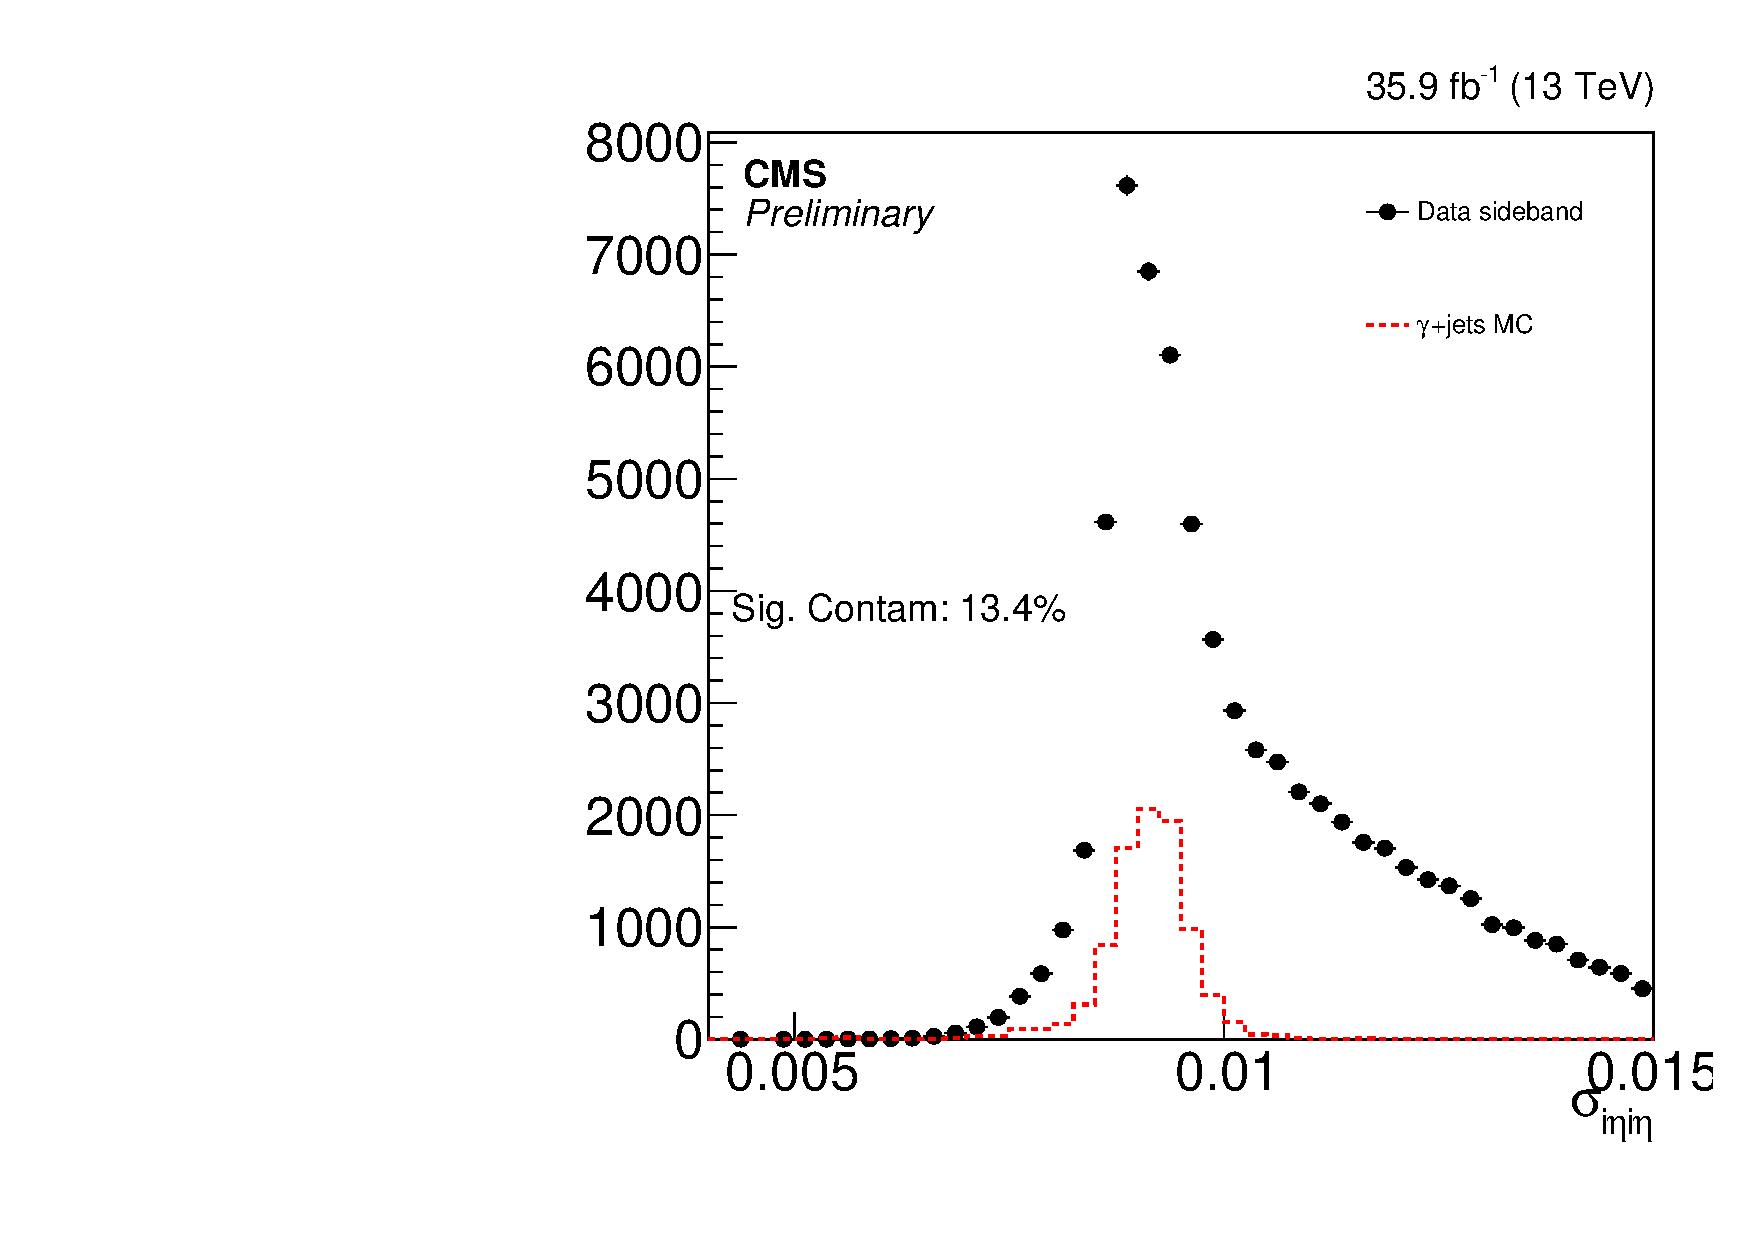
\includegraphics[]{Analysis/Figures/pvsf/sbcontam_nominal.pdf}
    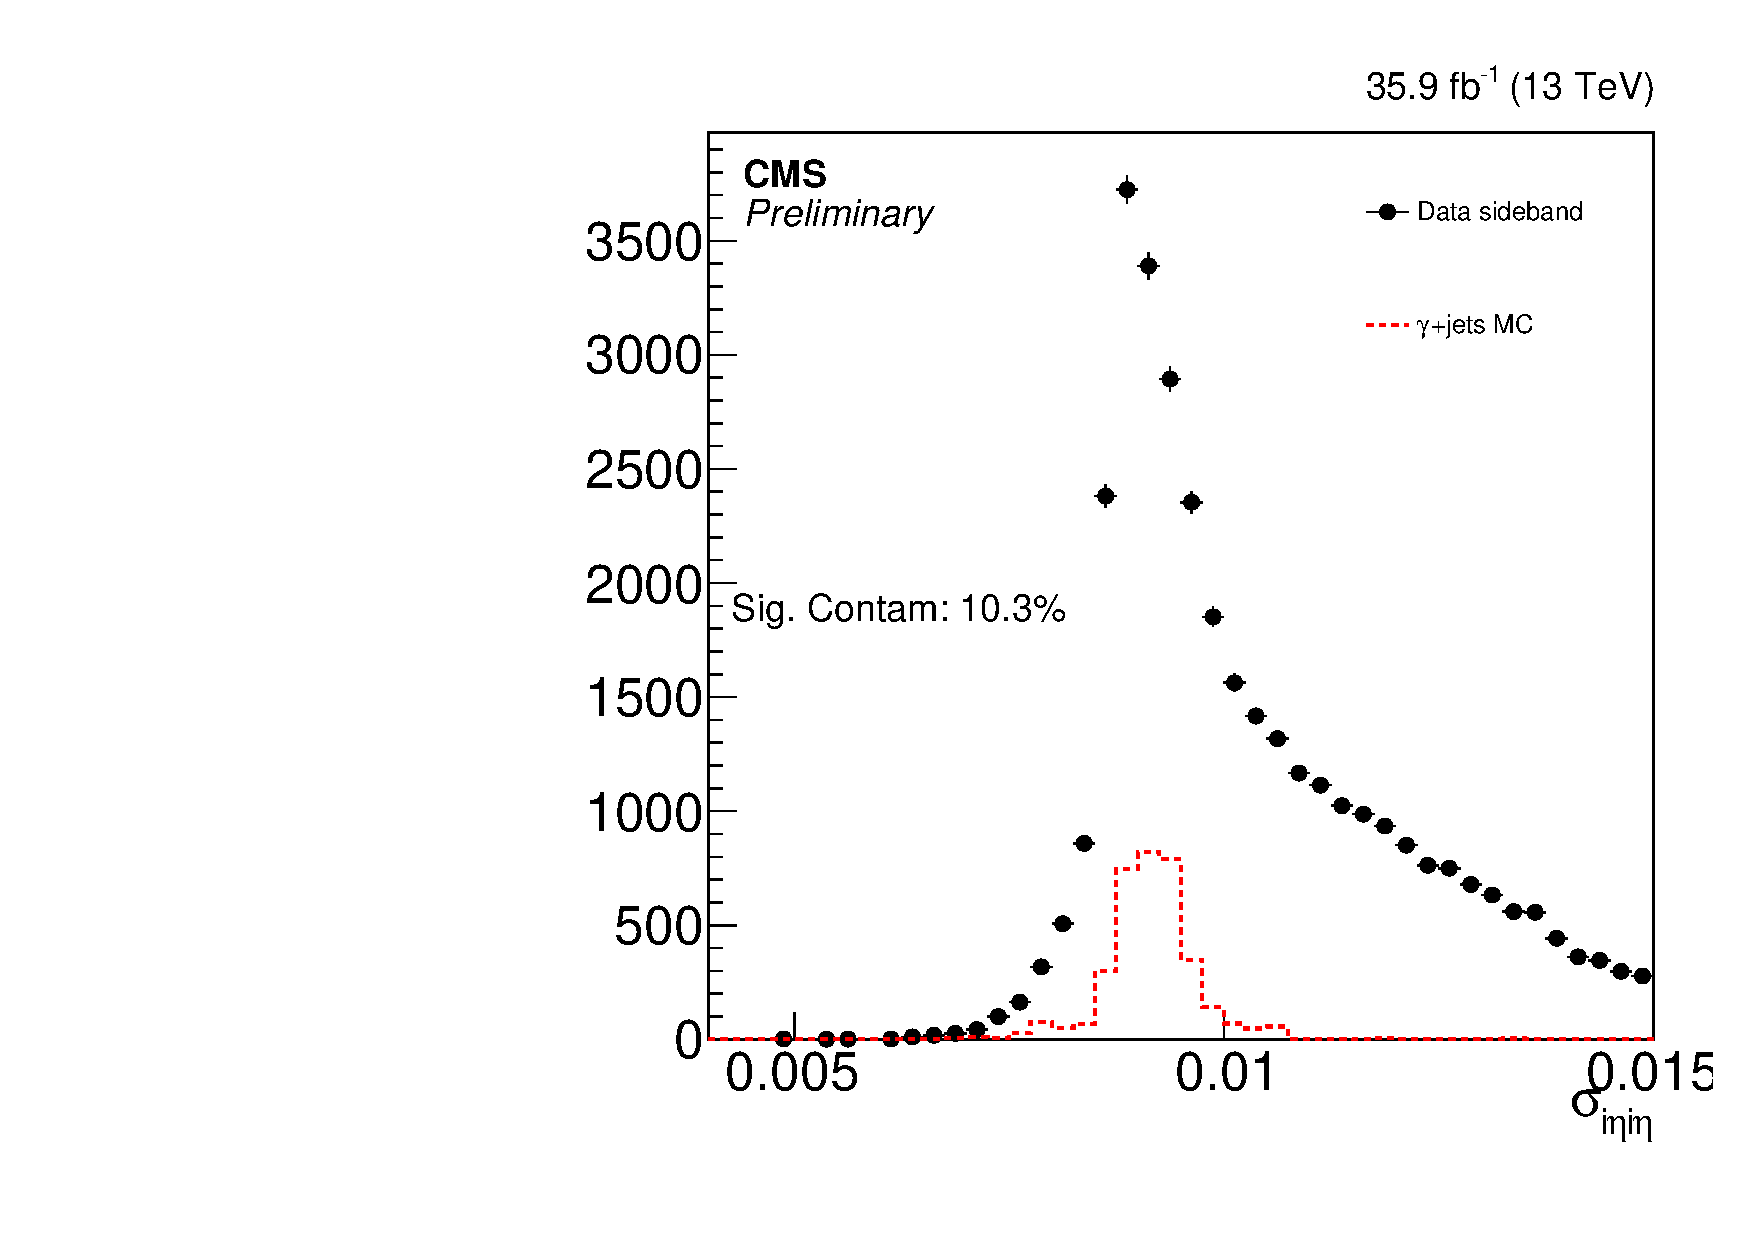
\includegraphics[]{Analysis/Figures/pvsf/sbcontam_far.pdf}
    }
  \caption{
    Signal contamination in the [3.5,5.0] (left), [5.0,7.5] (middle), and [7.5,9.0] (right) isolation sidebands.
  }
  \label{fig:impurity-signal-contamination}
\end{figure}

However, the hadronic background template, taken from the data control sample, has contributions from real photons with a \ICH\ value exceeding the ID requirements. 
The amount of this ``photon contamination'' depends on the sideband choice, but is non-zero even for a sideband with very large \ICH. 
As described below, we perform additional fits with the background templates from alternative sidebands $3.5\GeV < \ICH < 5\GeV$ (``near'') and $7.5\GeV < \ICH < 9\GeV$ (``far'') to assess the systematic uncertainty. 
The photon contamination of the nominal and far sideband is 10-15\%, and in the near sideband, it can go up to approximately 20\% (see Figure~\ref{fig:impurity-signal-contamination}).

To remove the photon contamination from the background templates, we start with the true photon shape in the sideband $h_{s^{'}}$, which differs from the signal template $h_{s}$ in the \ICH\ selection applied to the photons.
Then, we create a new background template $h_{b}^{\text{sub}}$ from the original background template $h_{b}$ by subtracting $h_{s^{'}}$. 
After normalization to unity, we obtain the expression
\begin{align}
  h_{b}^{\text{sub}}(\sieie) = \frac{h_{b}(\sieie) - S'/B \cdot h_{s'}(\sieie)}{1 - S'/B},
\end{align}
where $B$ is the number of photon candidates in the sideband and $S'$ is the number of true photons in the sideband.

To determine $S'$, we start with the number of true photons in the target sample, $f \cdot N$. 
We then scale this by the ratio of the relative fractions of true MC photons in the \ICH\ sideband $r_{\text{sb}}$ and in the signal region $r_{\text{sig}}$, giving us the expression
\begin{align}
  S' = f \cdot \frac{r_{\text{sb}}}{r_{\text{sig}}} \cdot N .
\end{align}

Going back to our original fit function and replacing $h_{b}$ with $h_{b}^{\text{sub}}$ gives us
\begin{align}
  P(f;\sieie) = f \cdot h_{s}(\sieie) + (1 - f) \times \frac{h_{b}(\sieie) - S'(f)/B \cdot h_{s'}(\sieie)}{1 - S'(f)/B},
\end{align}
which converges to the original fit function if $S' = 0$, \ie, if there is no photon contamination in the sideband. 
Note that $f$ is still the only free parameter for this new function as $S'$ only depends on $f$ and $r_{\text{sb}} / r_{\text{sig}}$ is set constant in the fit (see discussion of systematics for more detail).

\begin{figure}[htbp]
  \centering
  \resizebox{0.95\textwidth}{!}{
    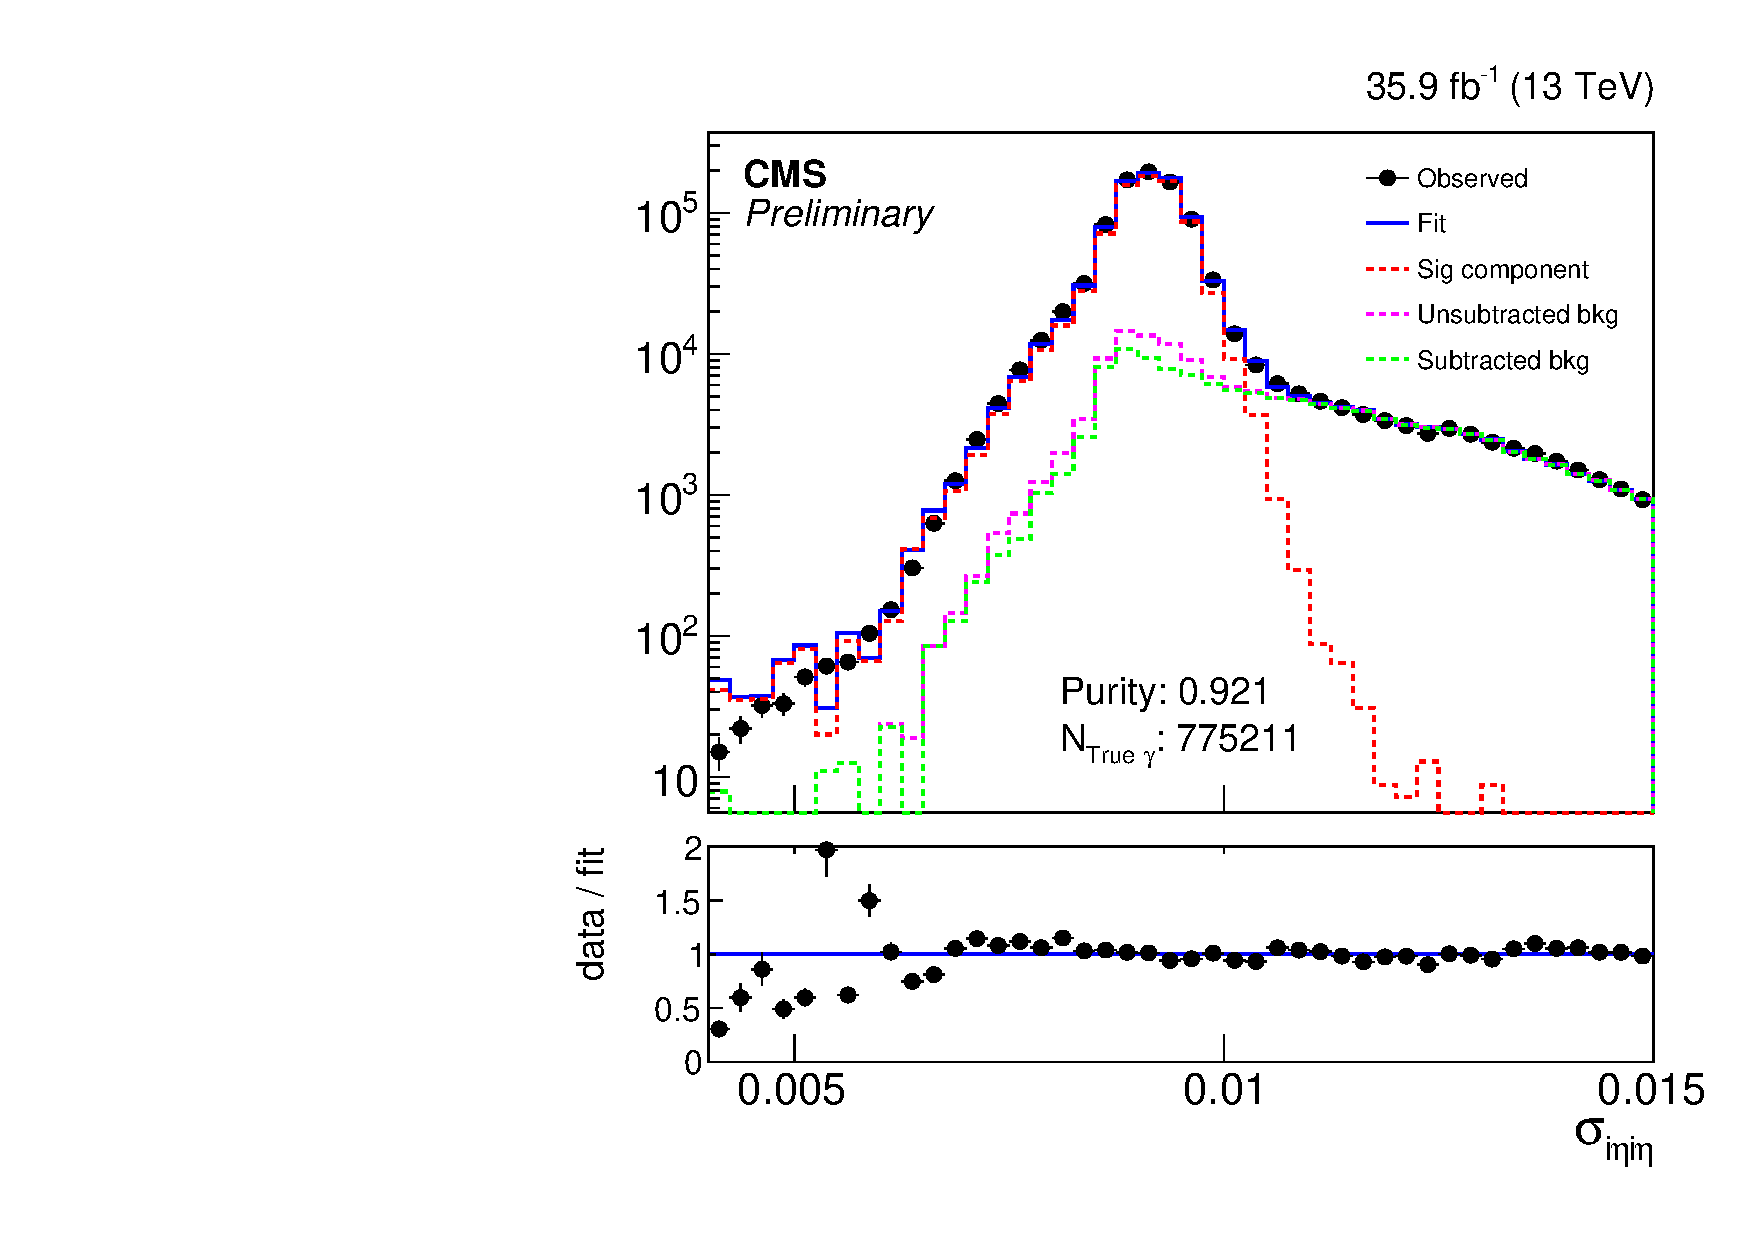
\includegraphics[]{Analysis/Figures/pvsf/ssfit_175_medium_near_logy.pdf}
    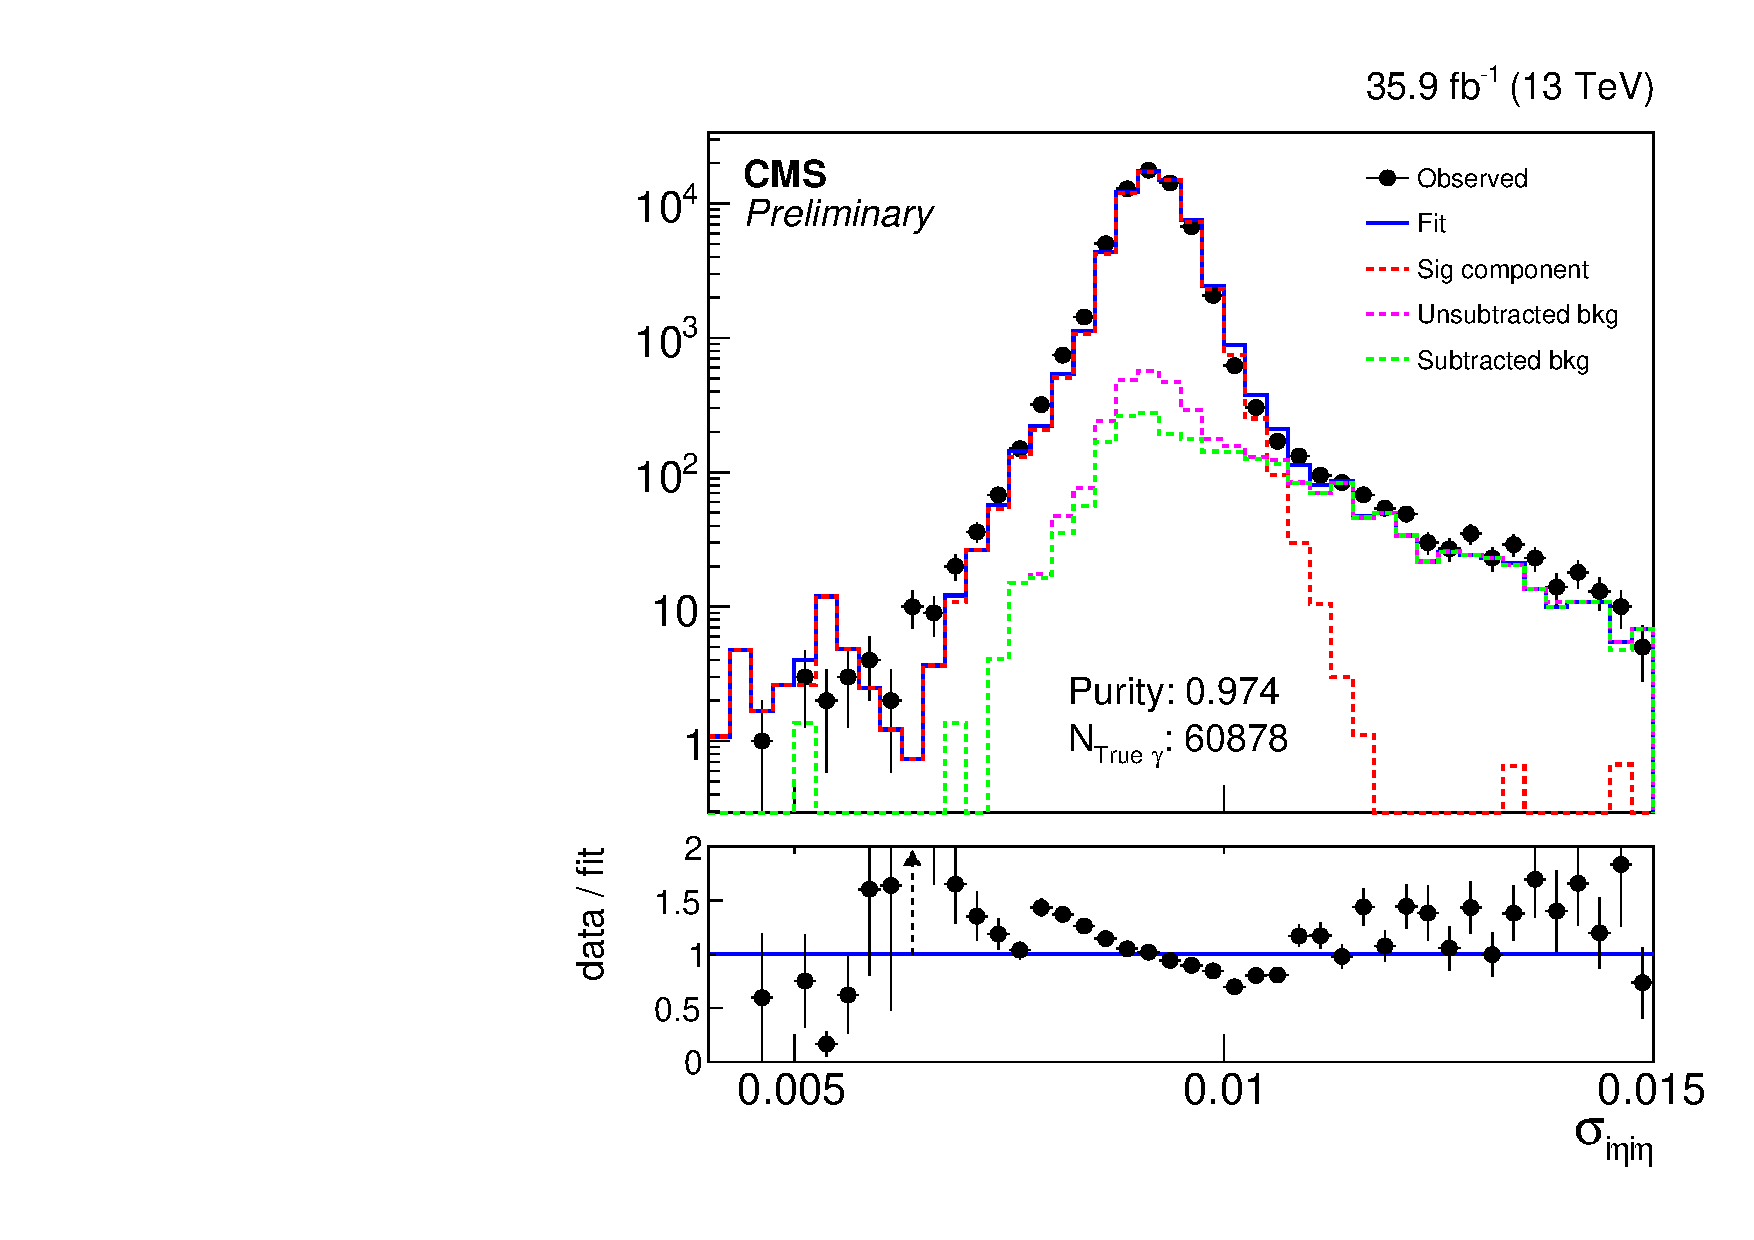
\includegraphics[]{Analysis/Figures/pvsf/ssfit_400_medium_near_logy.pdf}
  }
  \resizebox{0.95\textwidth}{!}{
    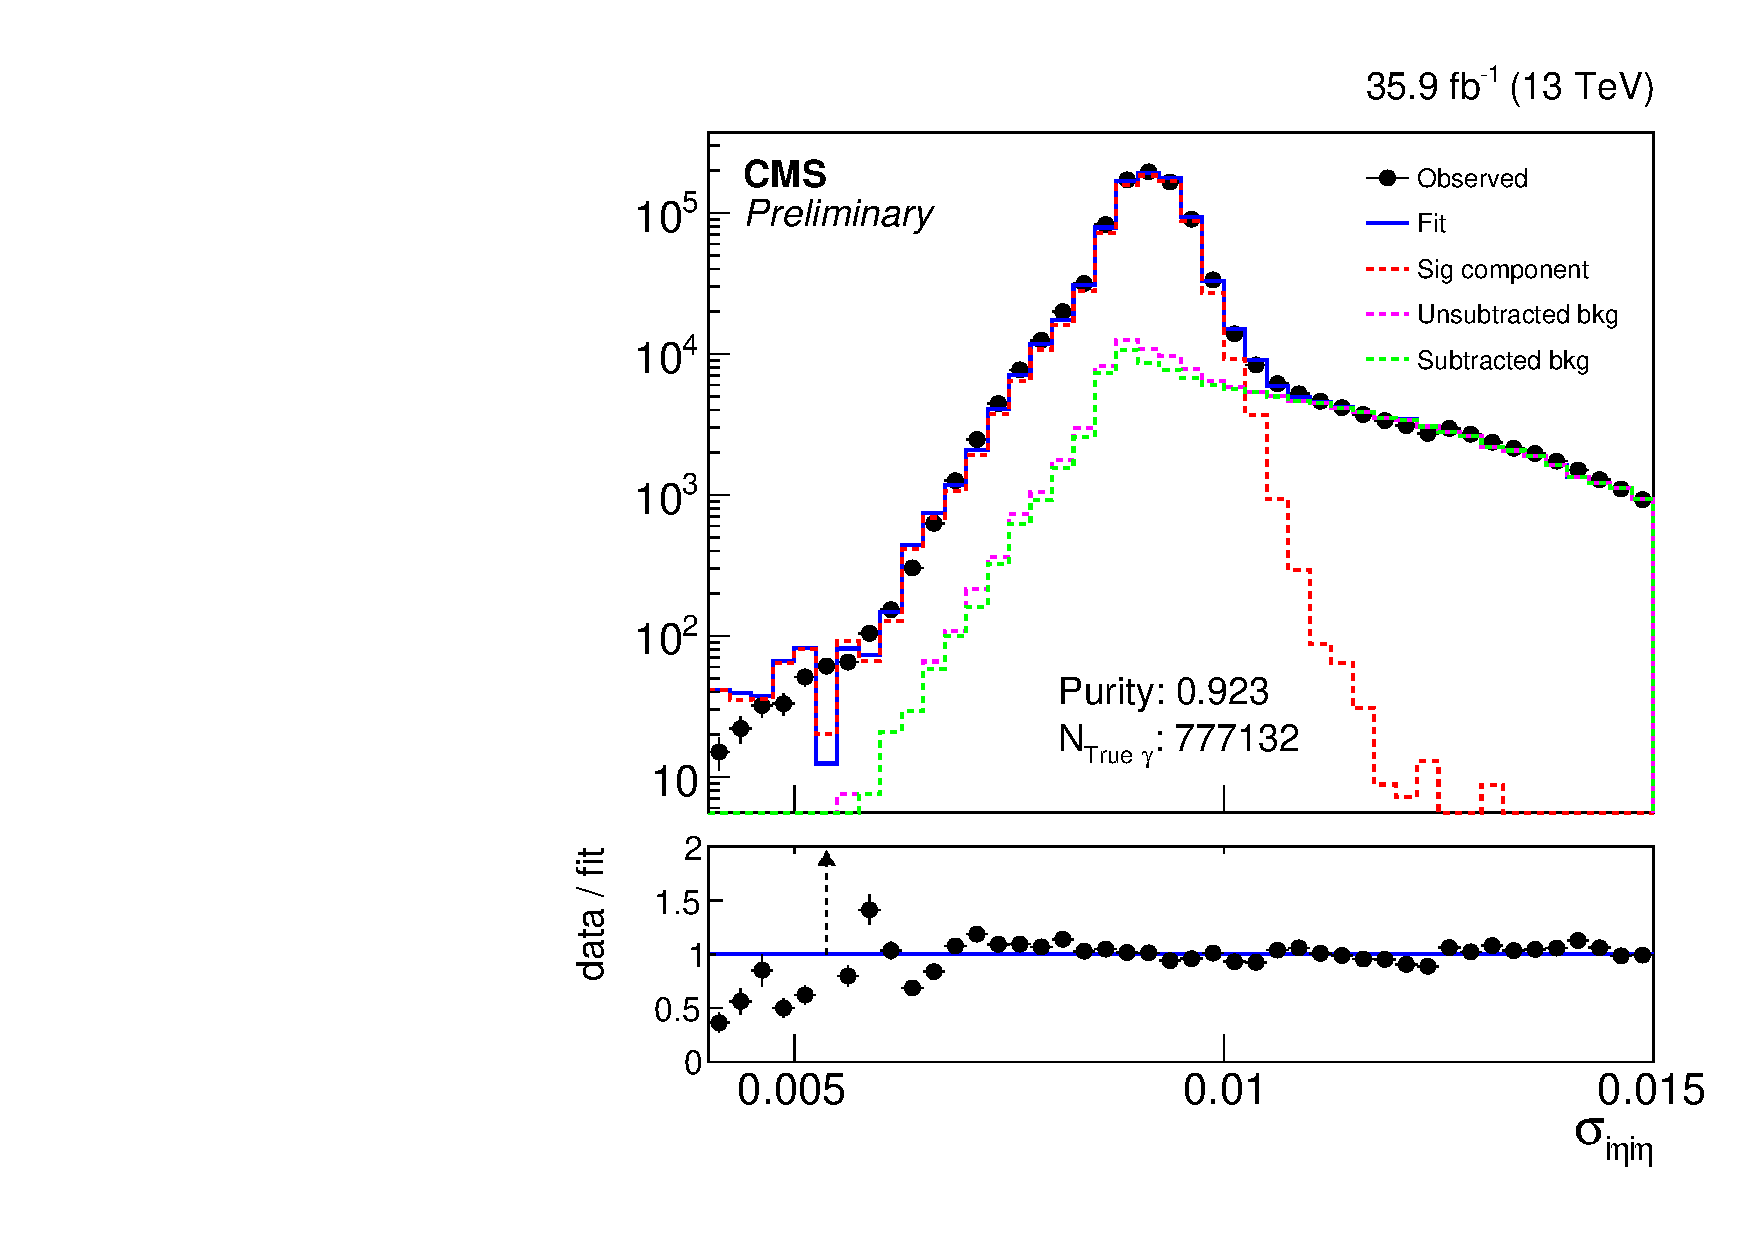
\includegraphics[]{Analysis/Figures/pvsf/ssfit_175_medium_nominal_logy.pdf}
    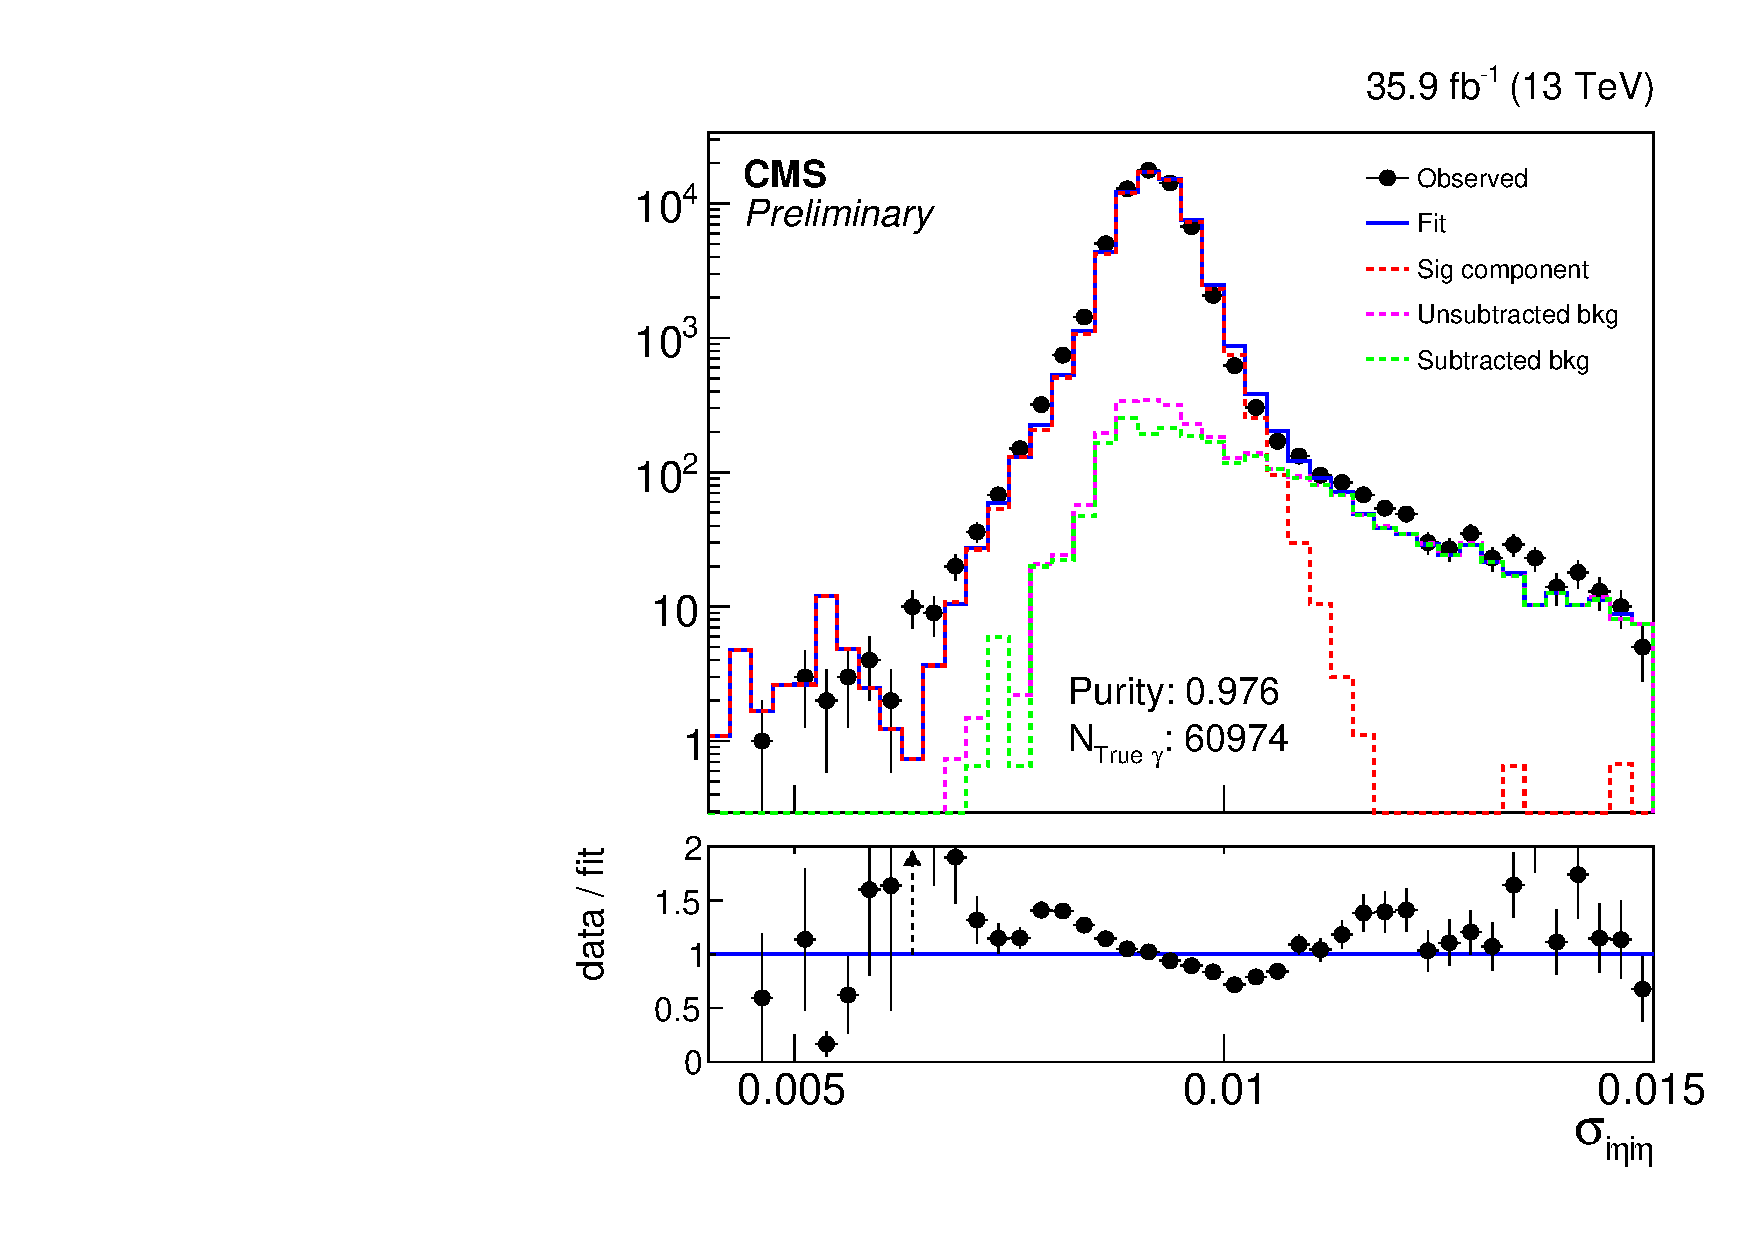
\includegraphics[]{Analysis/Figures/pvsf/ssfit_400_medium_nominal_logy.pdf}
  }
  \resizebox{0.95\textwidth}{!}{
    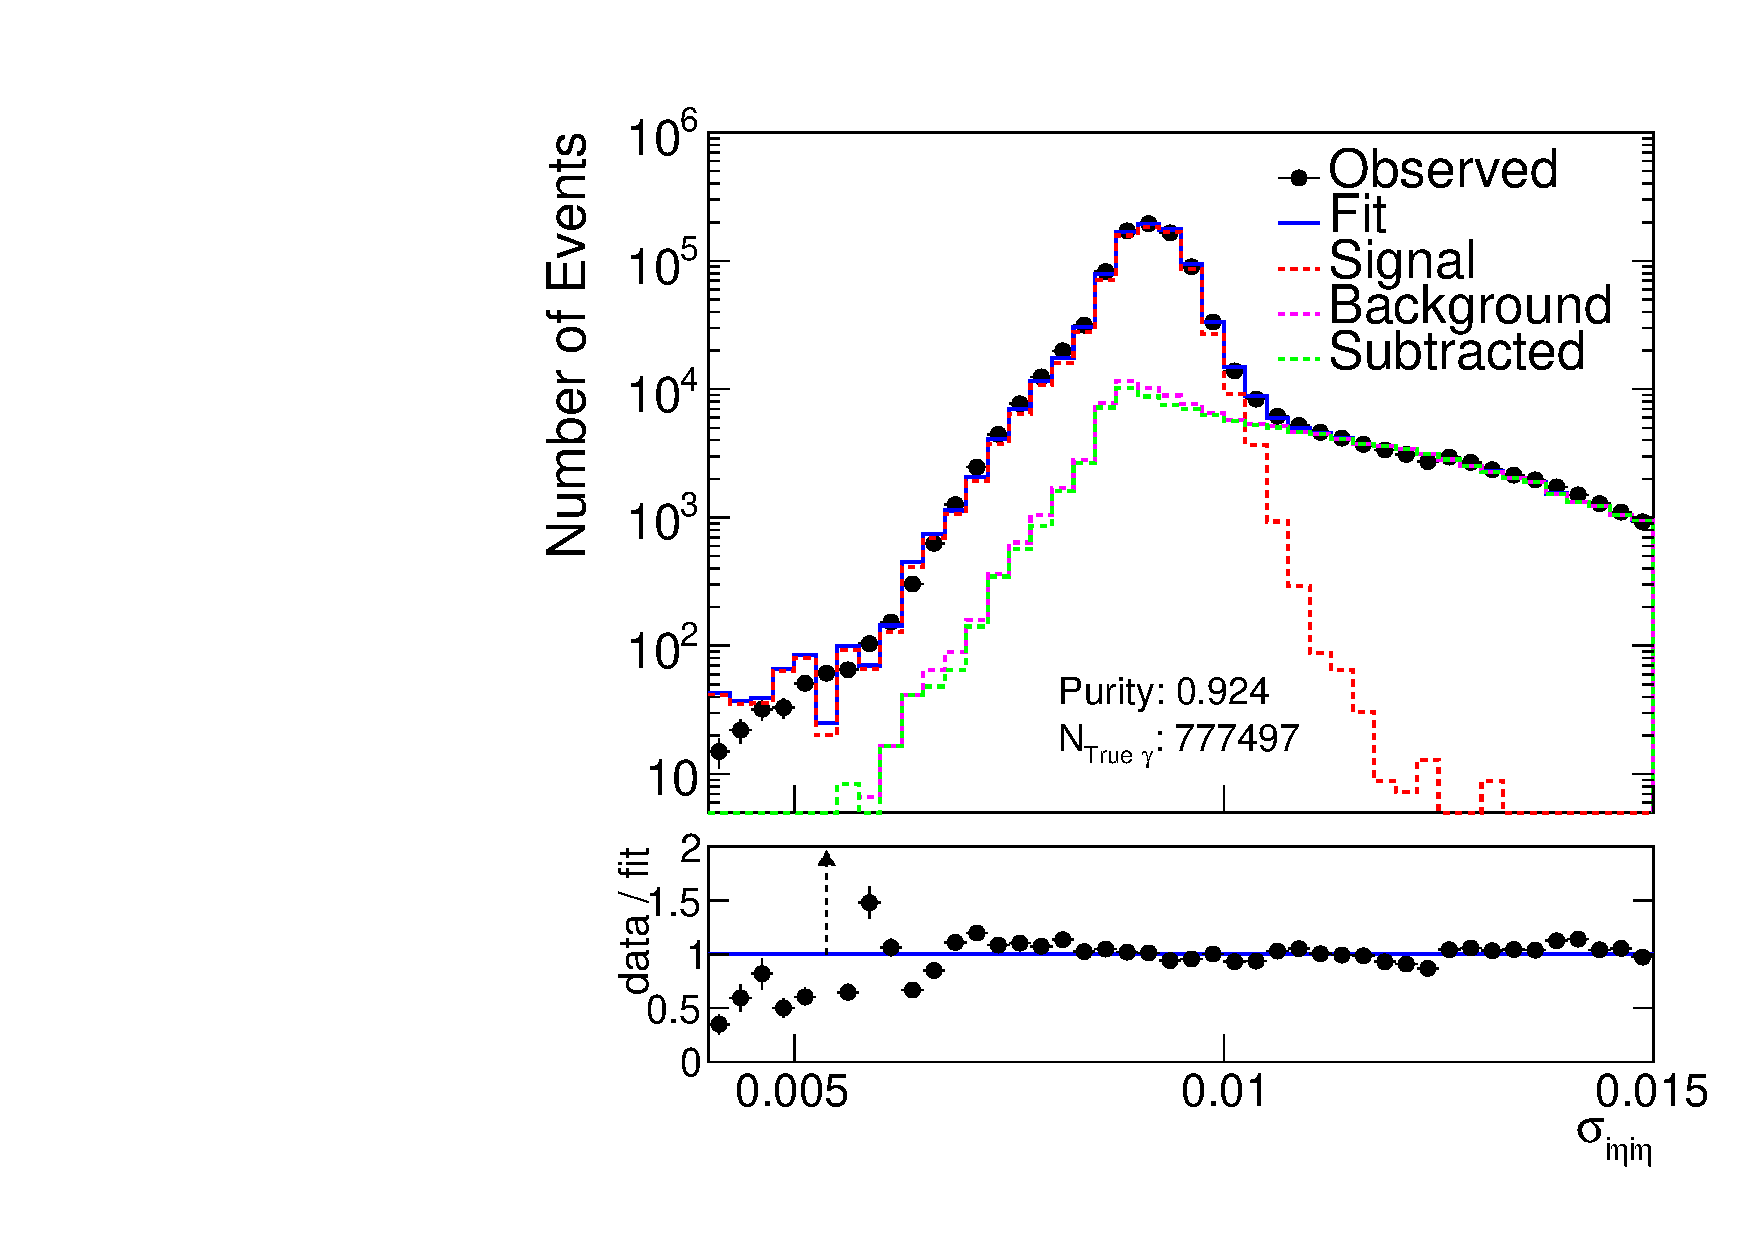
\includegraphics[]{Analysis/Figures/pvsf/ssfit_175_medium_far_logy.pdf}
    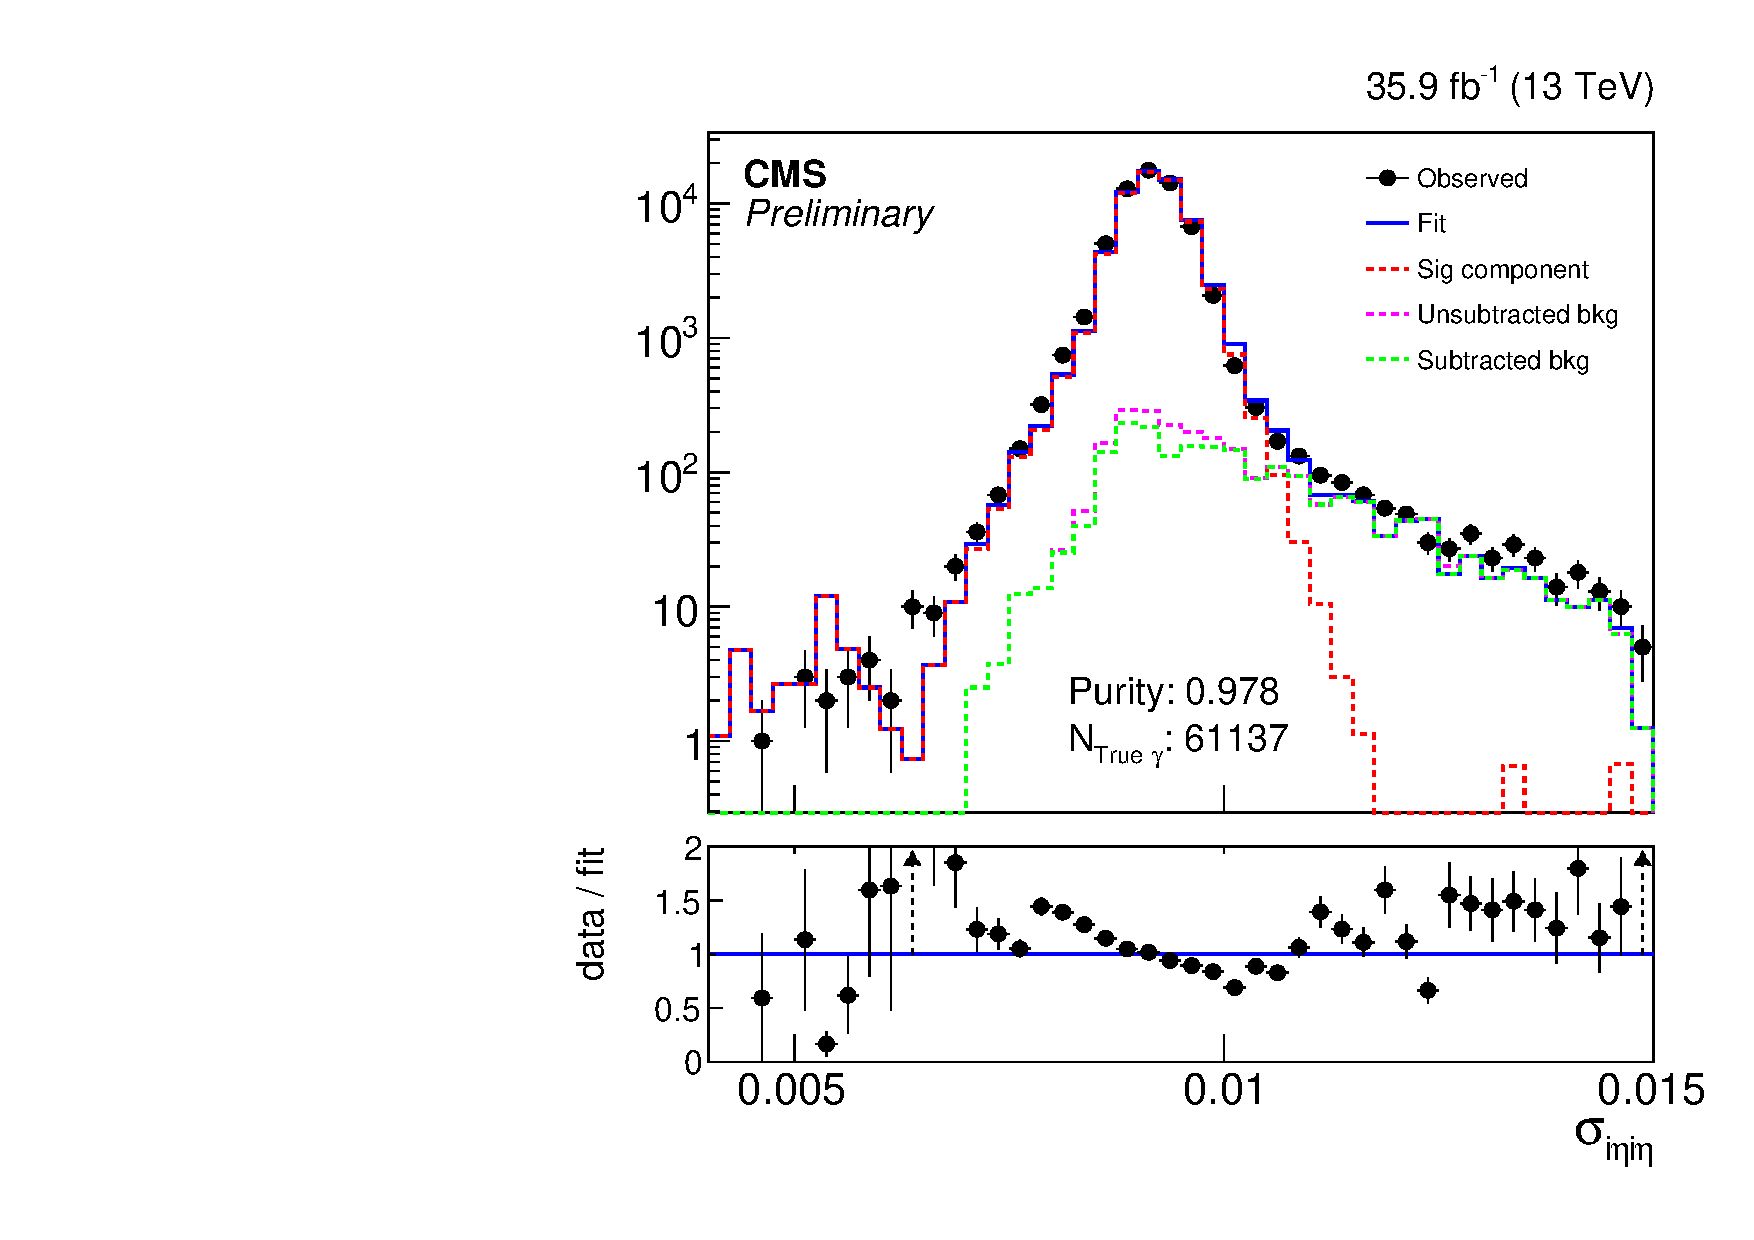
\includegraphics[]{Analysis/Figures/pvsf/ssfit_400_medium_far_logy.pdf}
  }
  \caption{
    Fits to the \sieie\ distributions for the [175, 200] (left) and [400,$\infty$) (right) \pt\ bins using the [3.5,5.0] (top), [5.0,7.5] (middle), and [7.5,9.0] (bottom) isolation sidebands.
      The blue solid line represents the full fit model, the red dashed line its signal component, and the green dashed line its background component.
    }
    \label{fig:impurity-sideband}
\end{figure}
\PH{plots need labels inside}

There are four main sources of systematic uncertainty for this measurement. 
The first comes from the sideband choice, as the relative rates of different types of fake photons varies with \ICH. 
The second comes from the true photon \ICH\ shape, as this is used to determine the normalization of true photons in the sideband. 
Currently, this shape is taken from MC and thus there is the potential to mismodel the effects of the underlying event and pile-up. 
The third comes from the true photon \sieie distribution. 
As we take this from MC as well, we can mismodel the signal template shape. 
Finally, at high \pt, we suffer from low yields in our \ICH\ sidebands, which leads fluctutations that negatively influence the fit.

The uncertainty due to sideband choice is the larger of the differences of the purities measured using the near and far sidebands versus the nominal sideband. 
Figure~\ref{fig:impurity-sideband} shows fits using the three sidebands for the [175,200] \pt\ bin on the left and for the [400,$\infty$) \pt\ bin on the right.

To measure the uncertainty due to the \ICH\ shape, we look at the \ICH\ for electrons in \Zee\ events in both data and MC. 
Using these distributions, we obtain a data/MC scale factor which we apply to the MC true photon \ICH\ distribution to obtain a scaled MC distribution. 
% This process is shown in Figure~\ref{fig:impurity-chiso}. 
Then, we recount the photons using this new distribution and take the difference in the values obtained using the raw MC and scaled MC distributions as a systematic uncertainty.

\iffalse
\begin{figure}[htbp]
  \centering
  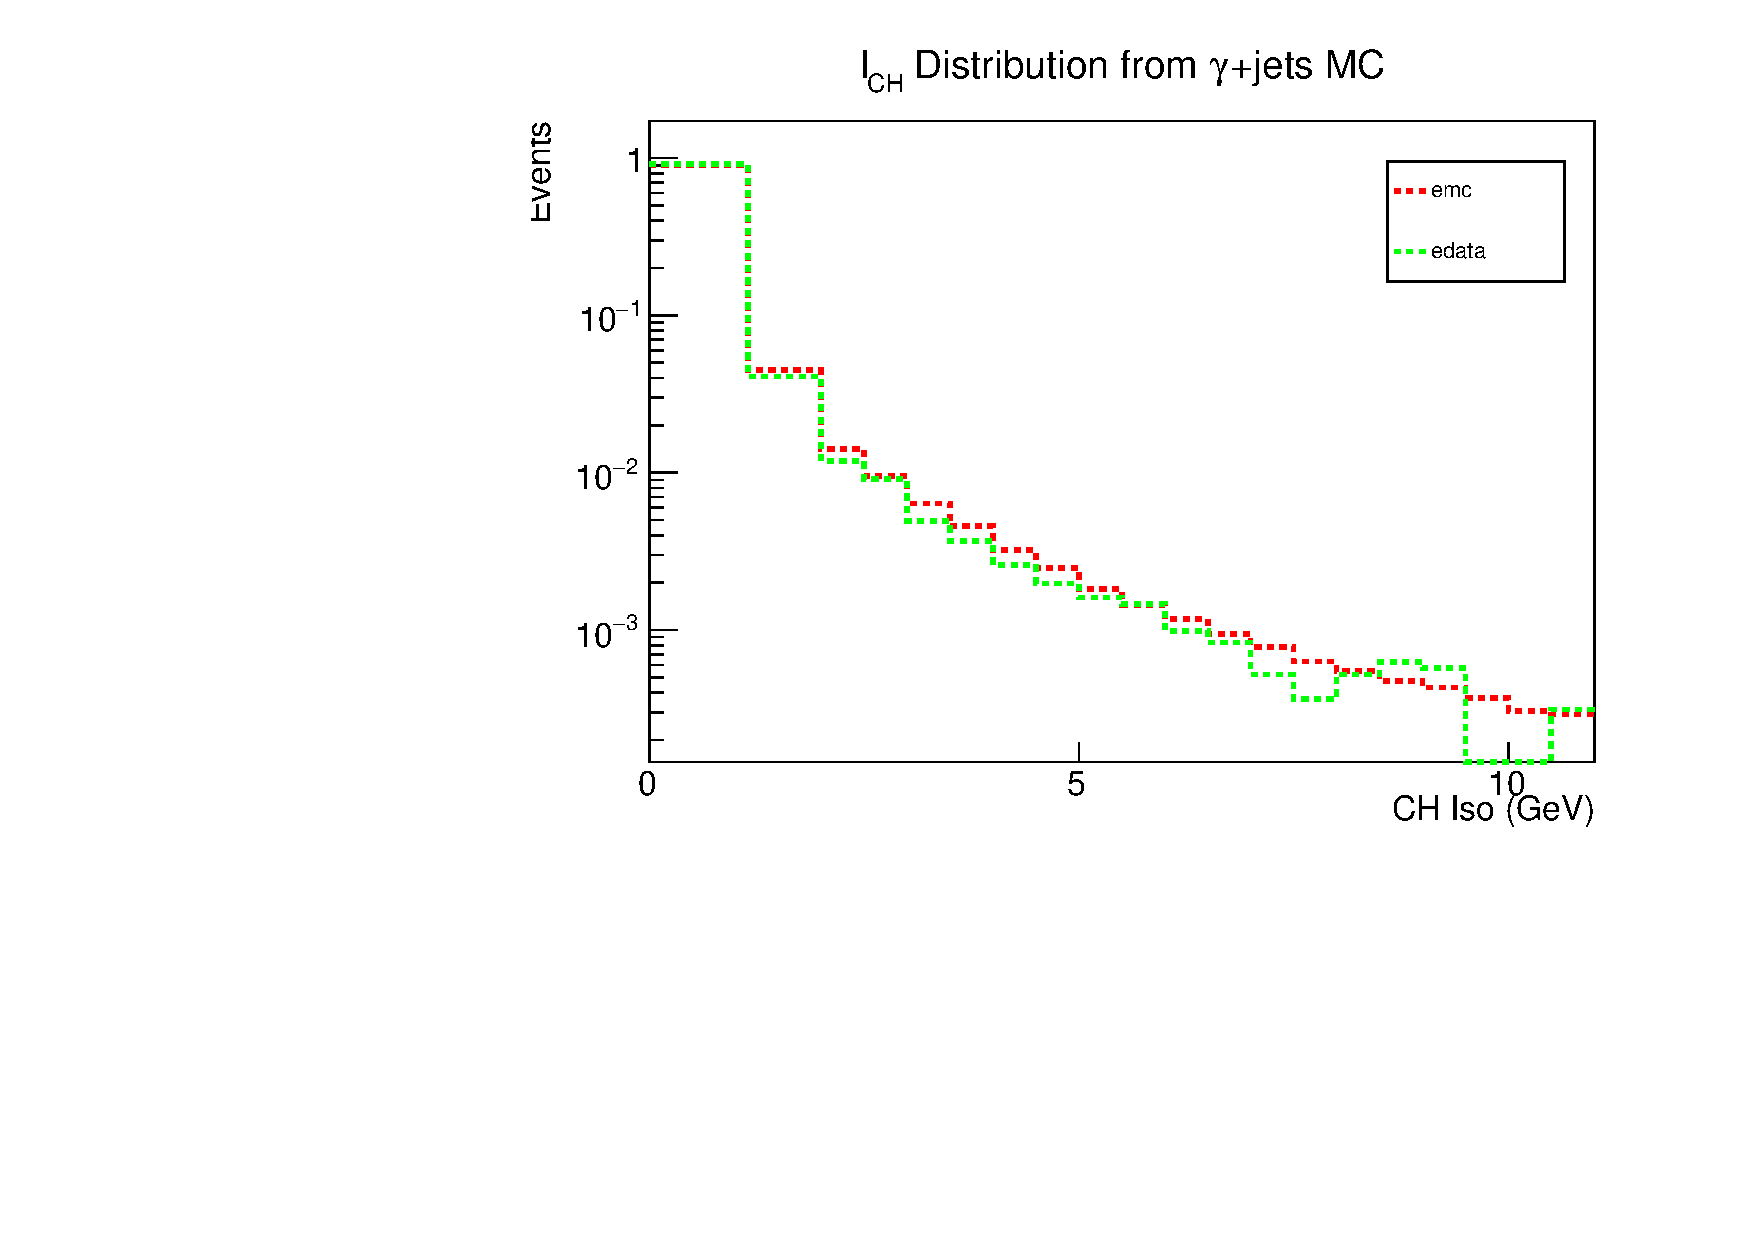
\includegraphics[width=0.45\textwidth]{Analysis/Figures/pvsf/chiso_electrons_logy.pdf}
  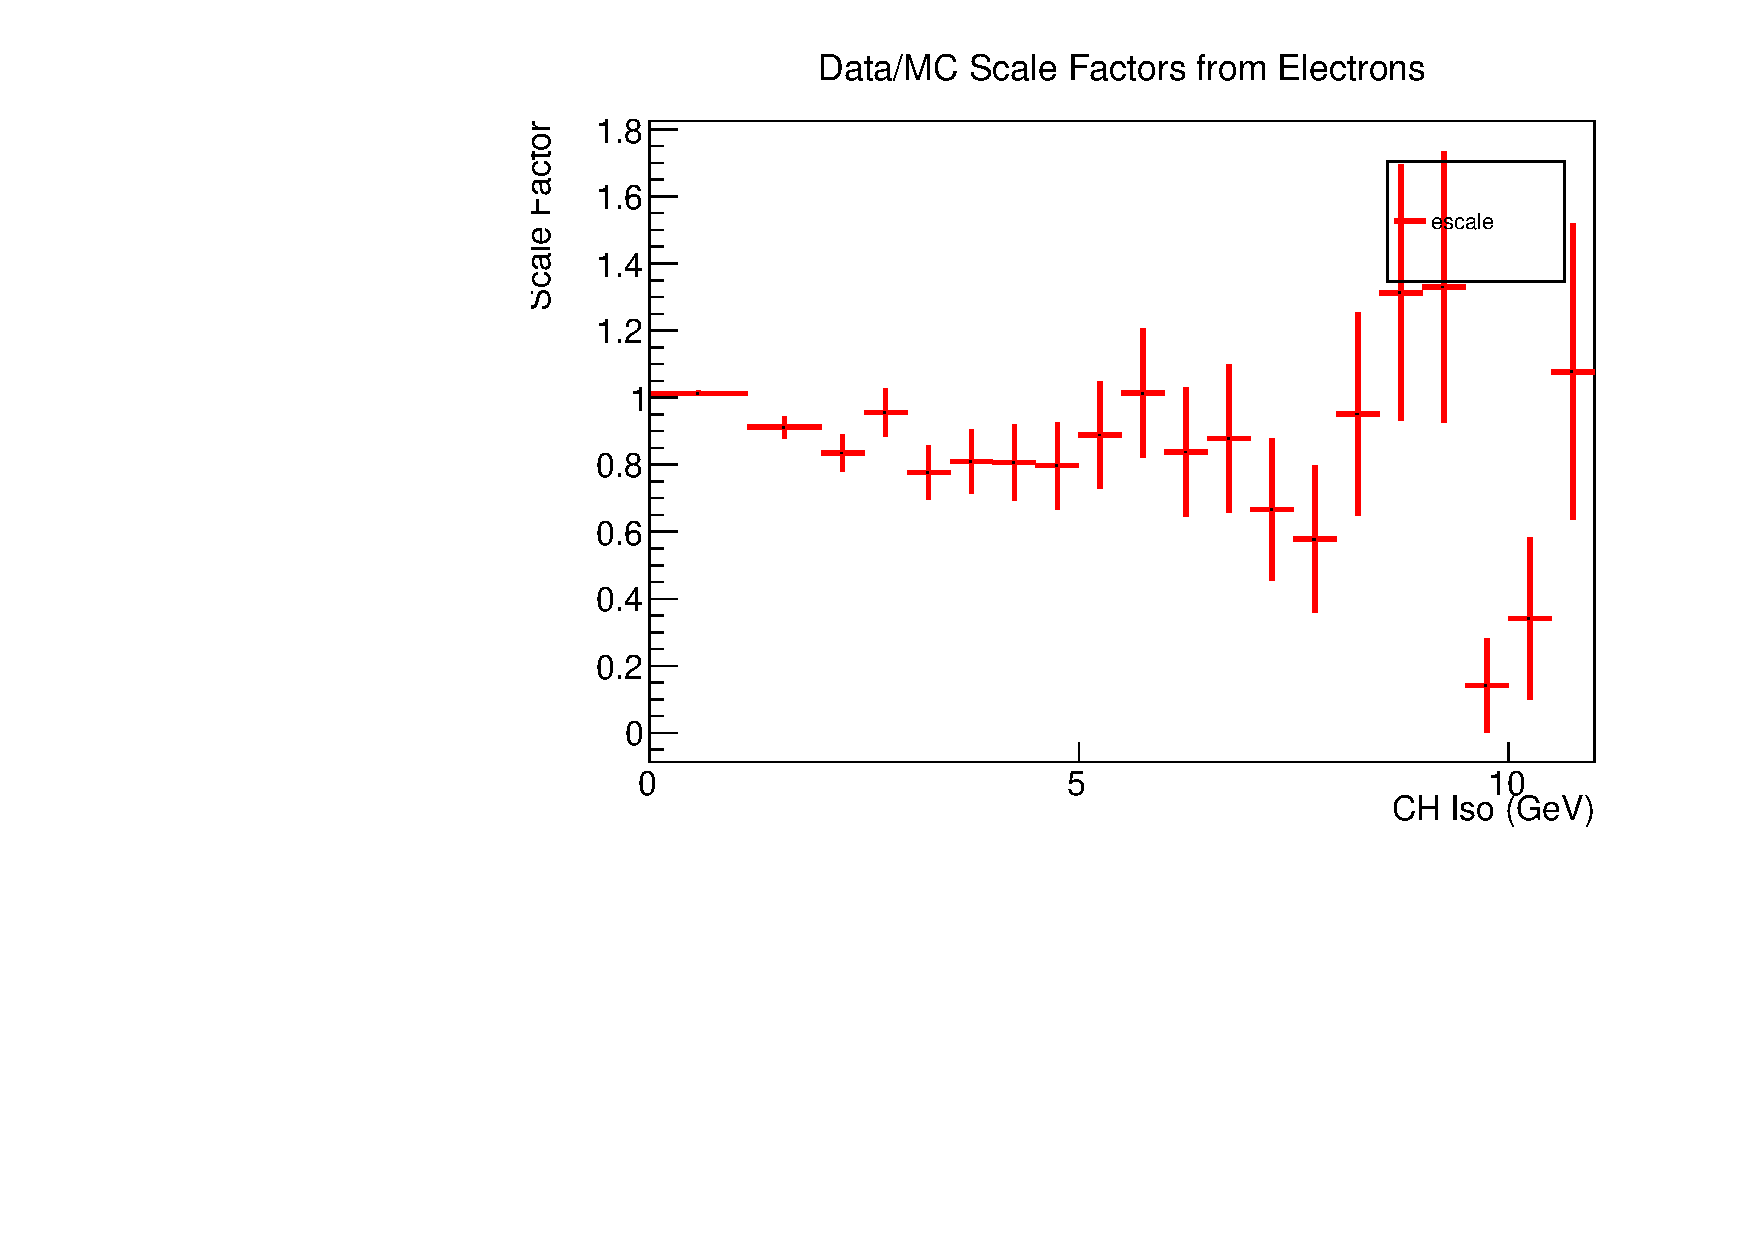
\includegraphics[width=0.45\textwidth]{Analysis/Figures/pvsf/chiso_scale.pdf}
  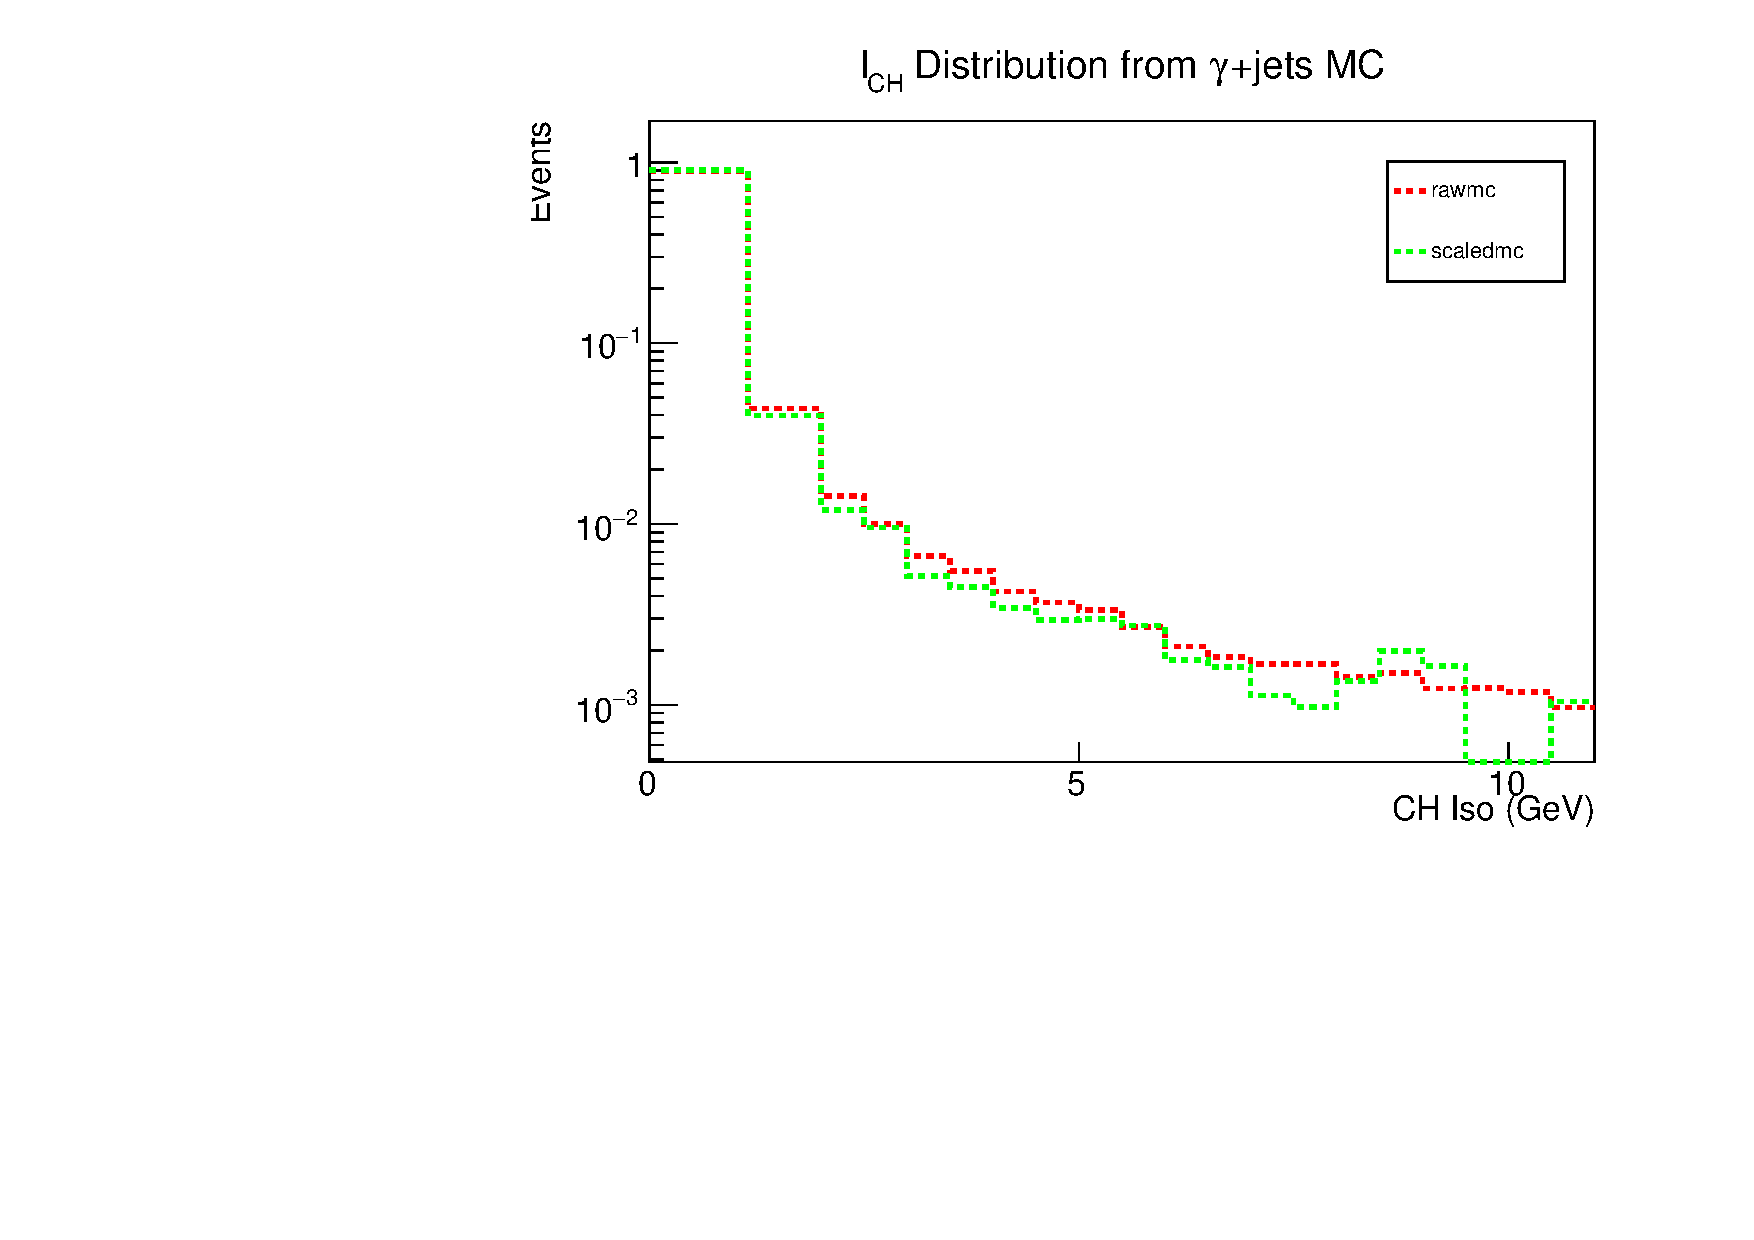
\includegraphics[width=0.45\textwidth]{Analysis/Figures/pvsf/chiso_photons_logy.pdf}
  \caption{
    Top left: \ICH\ distributions of electrons in data and MC in \Zee\ events.
    Top right: data/MC scale factor obtained from the electron \ICH\ distributions.
    Bottom: \ICH\ distributions of the MC photon objects used to estimate the amount of photon contamination in the background template, before and after applying the data/MC scale factor.
  }
  \label{fig:impurity-chiso}
\end{figure}
\fi

To measure the uncertainty due to the signal template \sieie\ shape, we look at the \sieie\ distributions for electrons from \Zee\ events in both data and MC.
Using these distributions, we obtain a data/MC scale factor which we apply to the MC true photon \sieie\ distribution to obtain a scaled MC distribution.
Then, we recount the photons using this new distribution and take the difference in the values obtained using the raw MC and scaled MC distributions as a systematic uncertainty. 
% The difference between fits with and without the \sieie\ scaling are shown in Figure~\ref{fig:impurity-sieie}.

\iffalse
\begin{figure}[htbp]
  \centering
  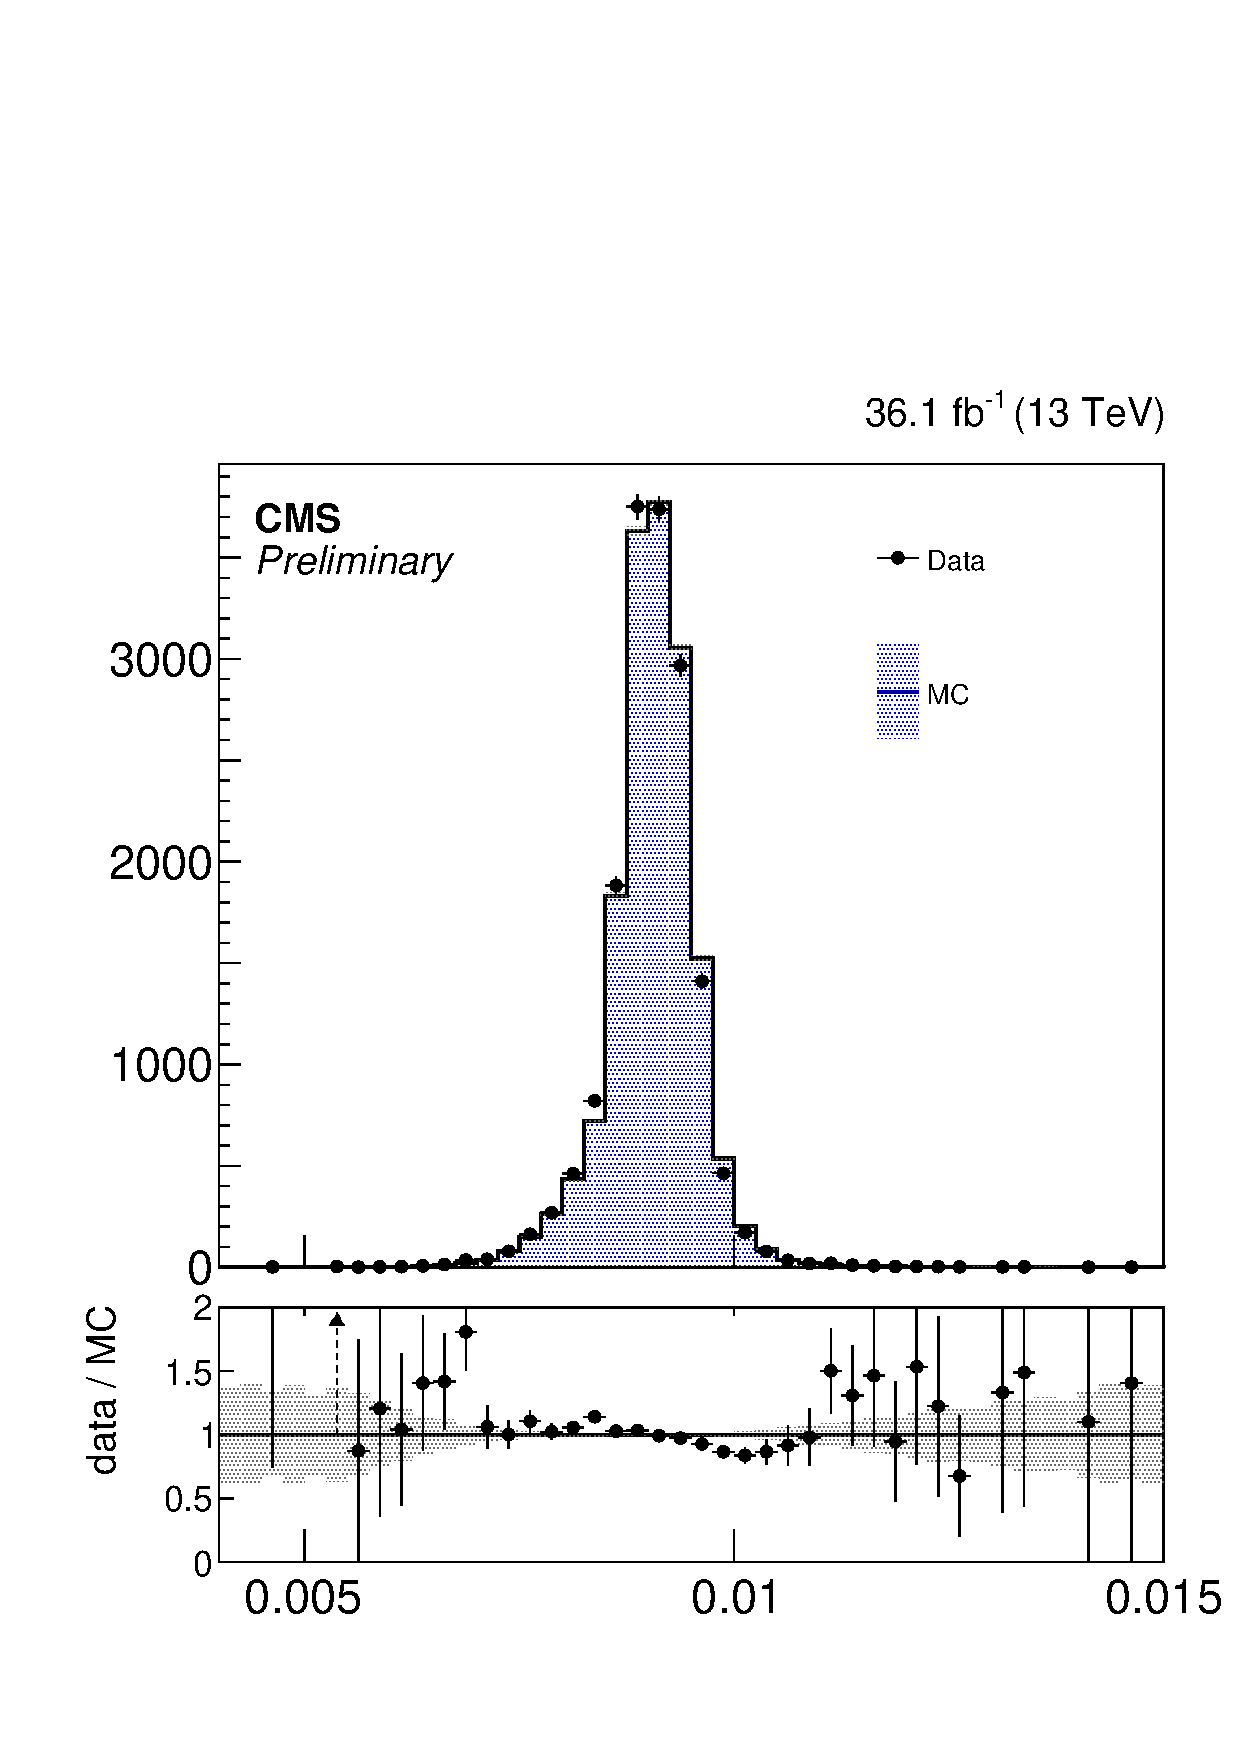
\includegraphics[width=0.45\textwidth]{Analysis/Figures/pvsf/sieie_ratio.pdf}
  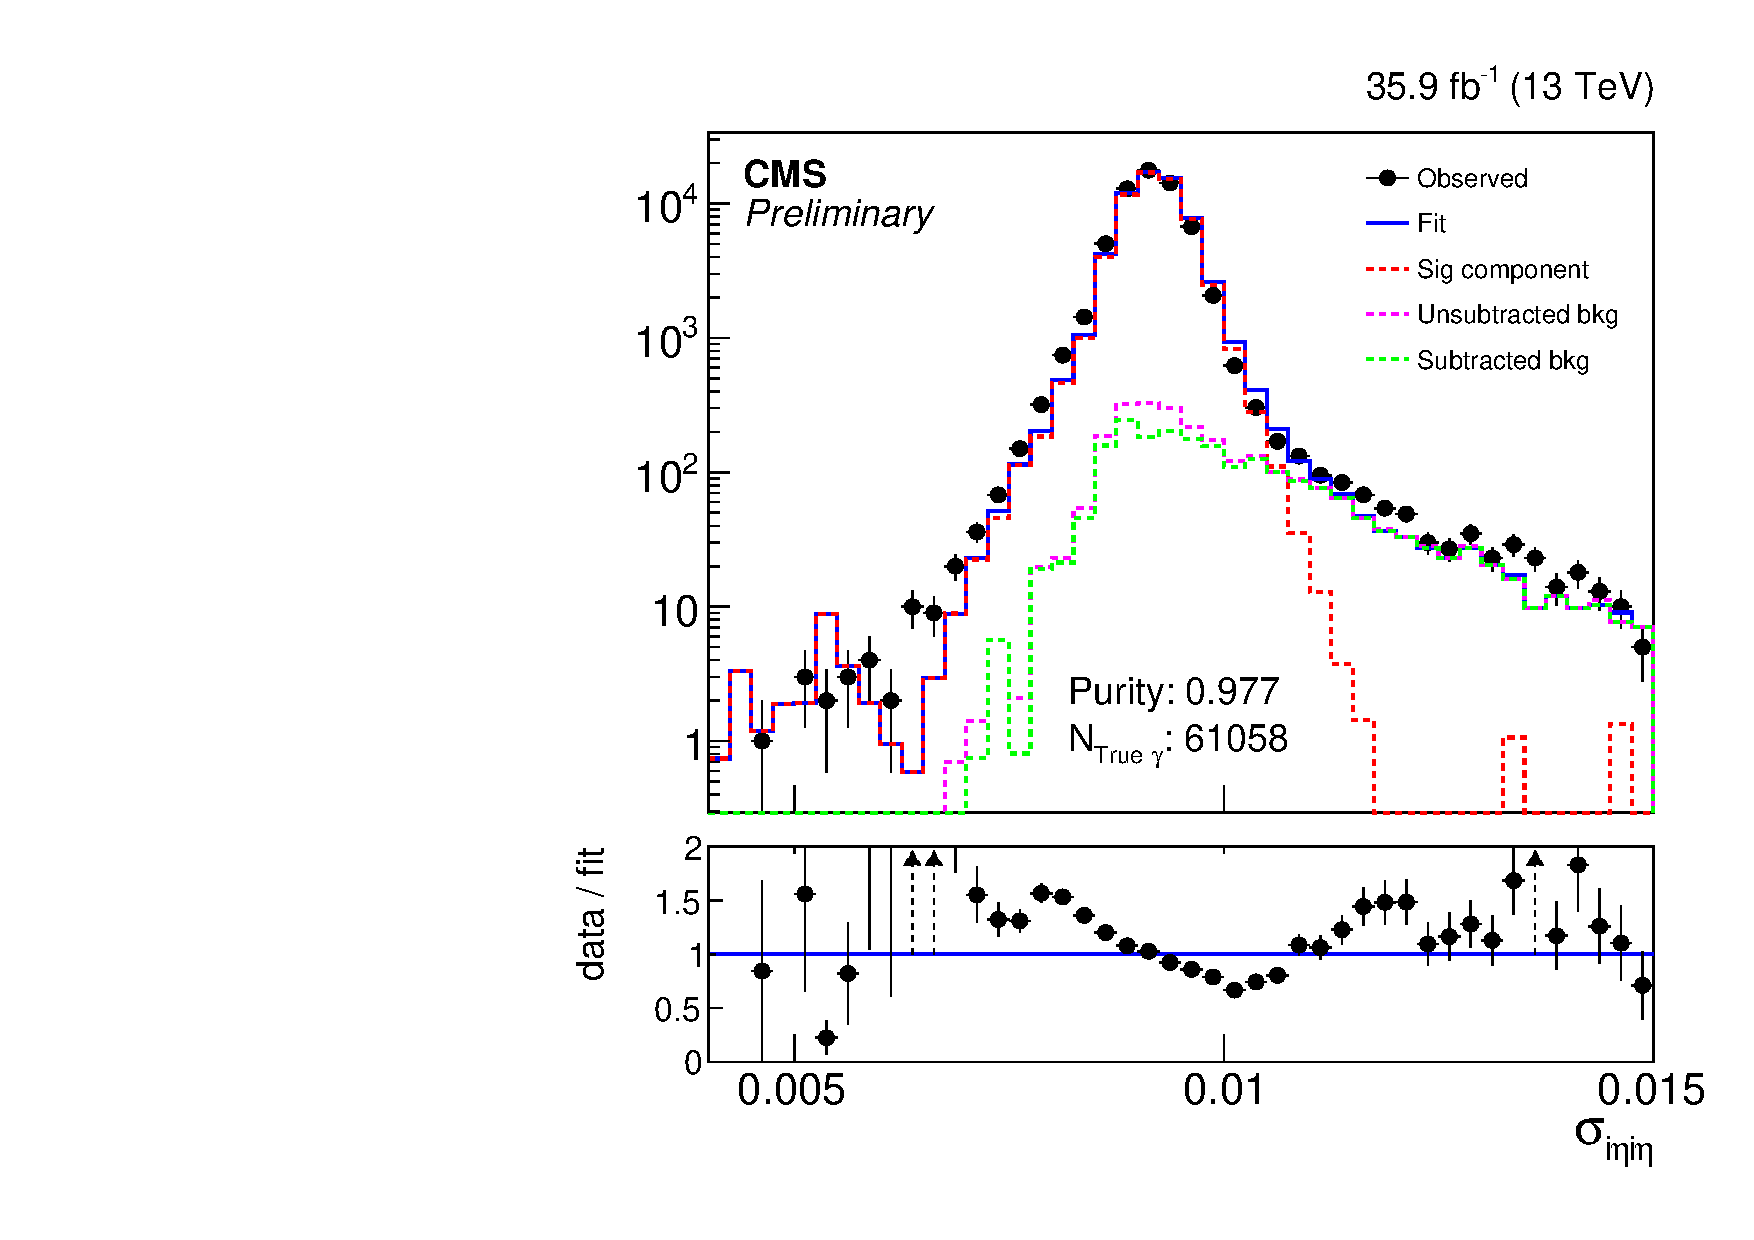
\includegraphics[width=0.45\textwidth]{Analysis/Figures/pvsf/ssfit_400_medium_shape_logy.pdf}
  \caption{
    Left: Comparison of \sieie\ distributions between data and MC in \Zee\ events. 
    Lower panel shows the data/MC \sieie\ scale factor.
    Right: Result of the fit with true-photon template with the data/MC \sieie\ scale factor applied to the true-photon template.
  }
  \label{fig:impurity-sieie}
\end{figure}
\fi

To estimate the uncertainty due to statistical fluctuations in our background templates, we generate toys from the background template from data. 
We then repeat the fit with each of these toys and plot the distribution of the difference between the purity value obtained from the toy templates versus the nominal template. 
We take the standard deviation of this distribution as a systematic uncertainty. % , shown in Figure~\ref{fig:impurity-toys},

\iffalse
\begin{figure}[htbp]
  \centering
  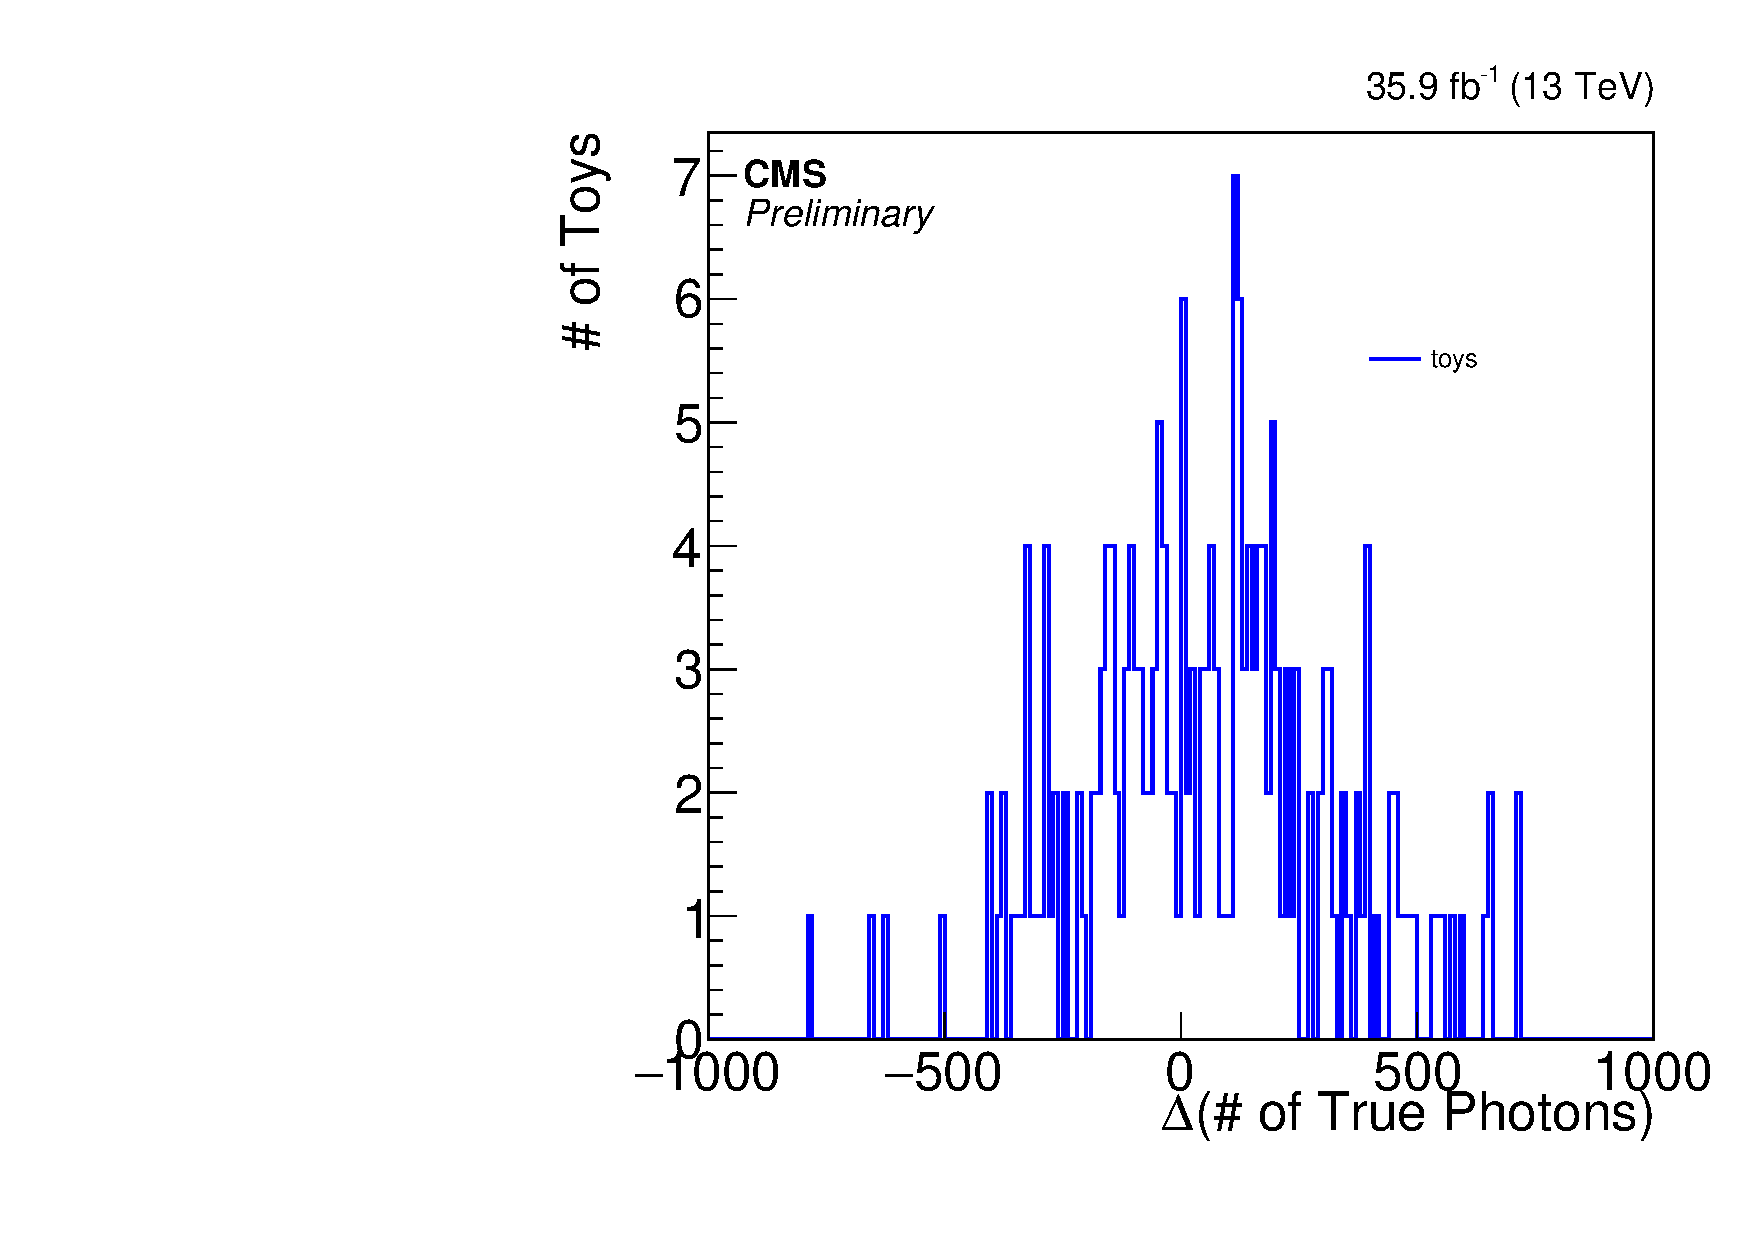
\includegraphics[width=0.45\textwidth]{Analysis/Figures/pvsf/ssfit_175_medium-pixel-monoph_toyyield_dist.pdf}
  \caption{
    Shift in true-photon yields, extracted from alternative fits varying the background template within its statistical uncertainty. 
    Nominal photon count in this specific \ETg\ bin is $6.64\times 10^{5}$.
  }
  \label{fig:impurity-toys}
\end{figure}
\fi

The values obtained for each systematic uncertainty on the true photon count of the denominator are shown in Table~\ref{tab:impurity-systs} in bins of \pt. 
The relative uncertainties on the numerator are similar, and in the
efficiency, each uncertainty source is considered as fully correlated.
\PH{Saying something is similar is not approporatie for a thesis. This
  All this information should be here}

\begin{table}[htbp]
  \centering
  \begin{tabular}{ c|c c c c }
    \pt\ Range & \multicolumn{4}{ |c }{Sources of Systematic Uncertainty} \\
    (GeV) & Sideband & \ICH\ Shape & Signal Shape & Bgkd. Stats \\
    \hline
    (175, 200)  & 0.09 & 0.18 & 0.05 & 0.04 \\
    (200, 250)  & 0.01 & 0.16 & 0.06 & 0.03 \\
    (250, 300)  & 0.14 & 0.16 & 0.06 & 0.05 \\
    (300, 350)  & 0.12 & 0.16 & 0.07 & 0.08 \\
    (350, 400)  & 0.23 & 0.11 & 0.05 & 0.10 \\
    (400, $\infty$)  & 0.27 & 0.09 & 0.05 & 0.05
  \end{tabular}
  \caption{Relative uncertainties on the estimated number of true photons in the denominator sample.}
  \label{tab:impurity-systs}
\end{table}

The MC efficiency of the \Pgg-specific ID is determined by counting the number of truth-matched photons passing the \egamma\ part of the ID and the full ID. 
However, there is a complication, the \gj\ region in data has approximately 5\% contamination from electrons before applying the pixel veto, as shown in Figure~\ref{fig:pvsf_contam}. 
To replicate this effect in the MC, we combine appropriately cross-section weighted \gj, \wj, and \ttbar\ samples and truth match to both electrons and photons. 
Additionally, to account for the NLO cross-section ratio uncertainties
with respect to \gj\ at this \pt\ range, we apply a 14\% uncertainty
on the \wj\ and \ttbar\ yields, where the specific value comes from
the uncertainty on the \gj\ to \wj\ ratio in the monojet
analysis~\cite{}. \PH{Missing citation}
This uncertainty is uncorrelated between the numerator and denominator as a negligible amount of electron events survive the pixel veto.

\begin{figure}[htbp]
  \centering
  \resizebox{\textwidth}{!}{
    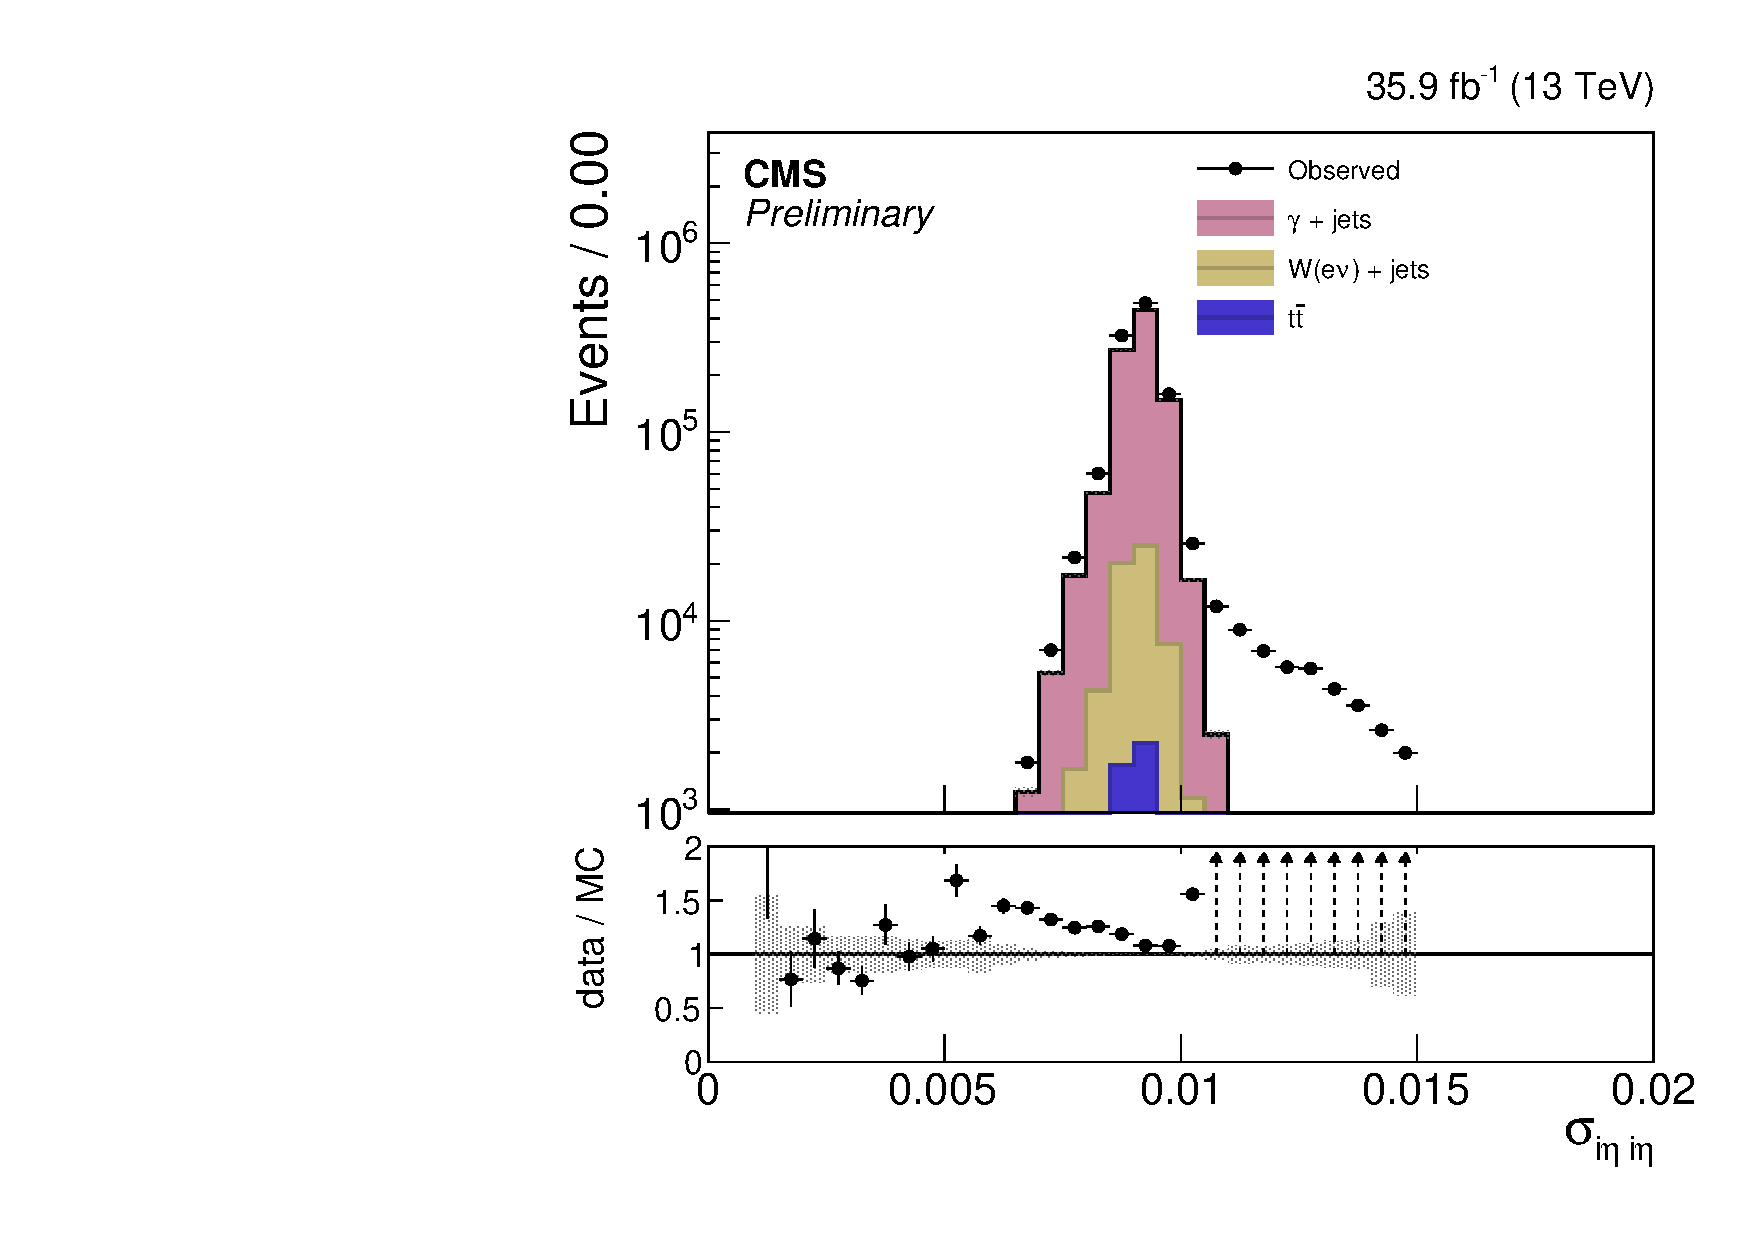
\includegraphics[]{Analysis/Figures/pvsf/gjets_sieie.pdf}
    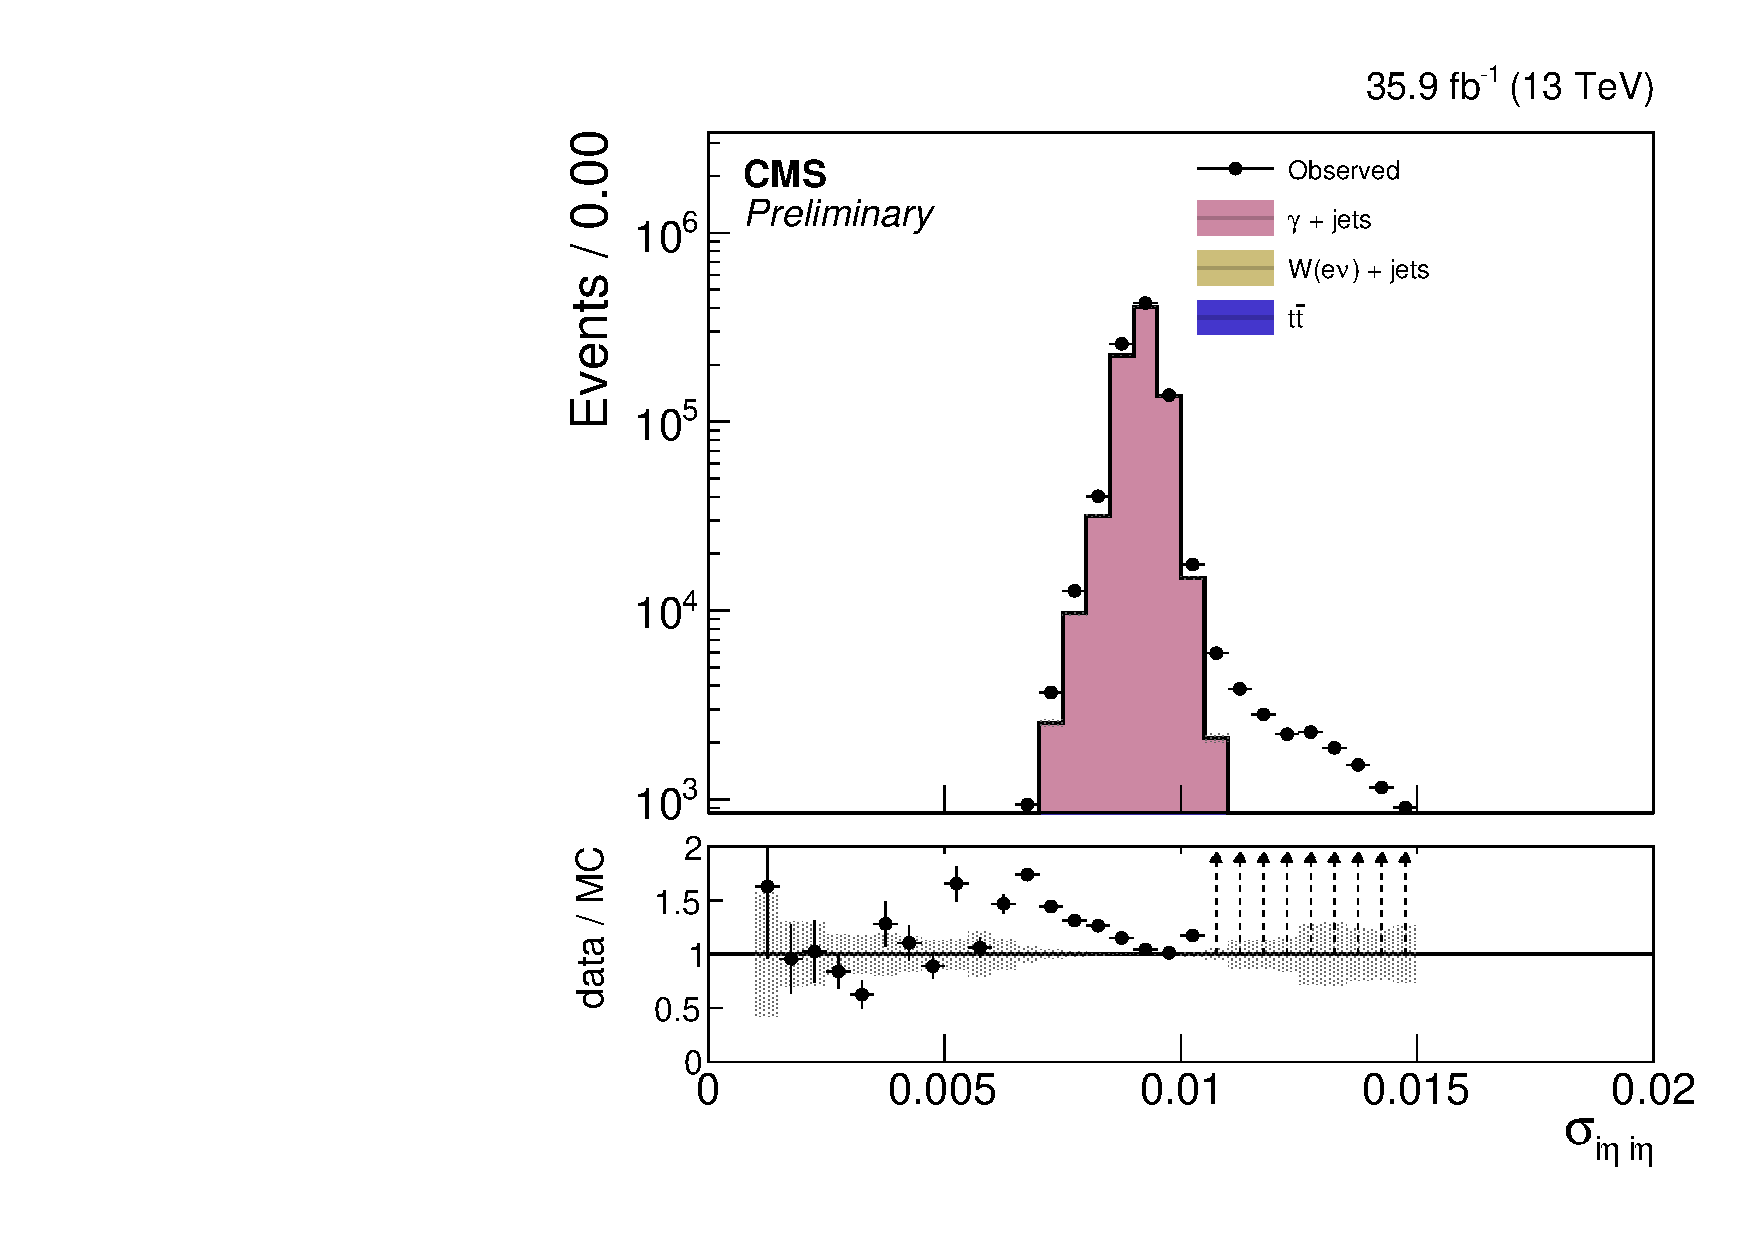
\includegraphics[]{Analysis/Figures/pvsf/gjets_sieiePixelVeto.pdf}
  }
  \caption{
    Electron contamination in \gj\ region before (left) and after (right) applying the pixel seed veto.
  }
  \label{fig:pvsf_contam}
\end{figure}
 
The data efficiency, MC efficiency, and the scale factor for the \Pgg-specific ID as a function of \pt\ are shown in Figure~\ref{fig:pvsf_results}. 
As there is no significant trend in the scale factor as a function of \pt, we apply a flat scale factor of $0.9840 \pm 0.0090$ for all of the MC-based background and signal models in the analysis.

\begin{figure}[htbp]
  \centering
  \resizebox{\textwidth}{!}{
    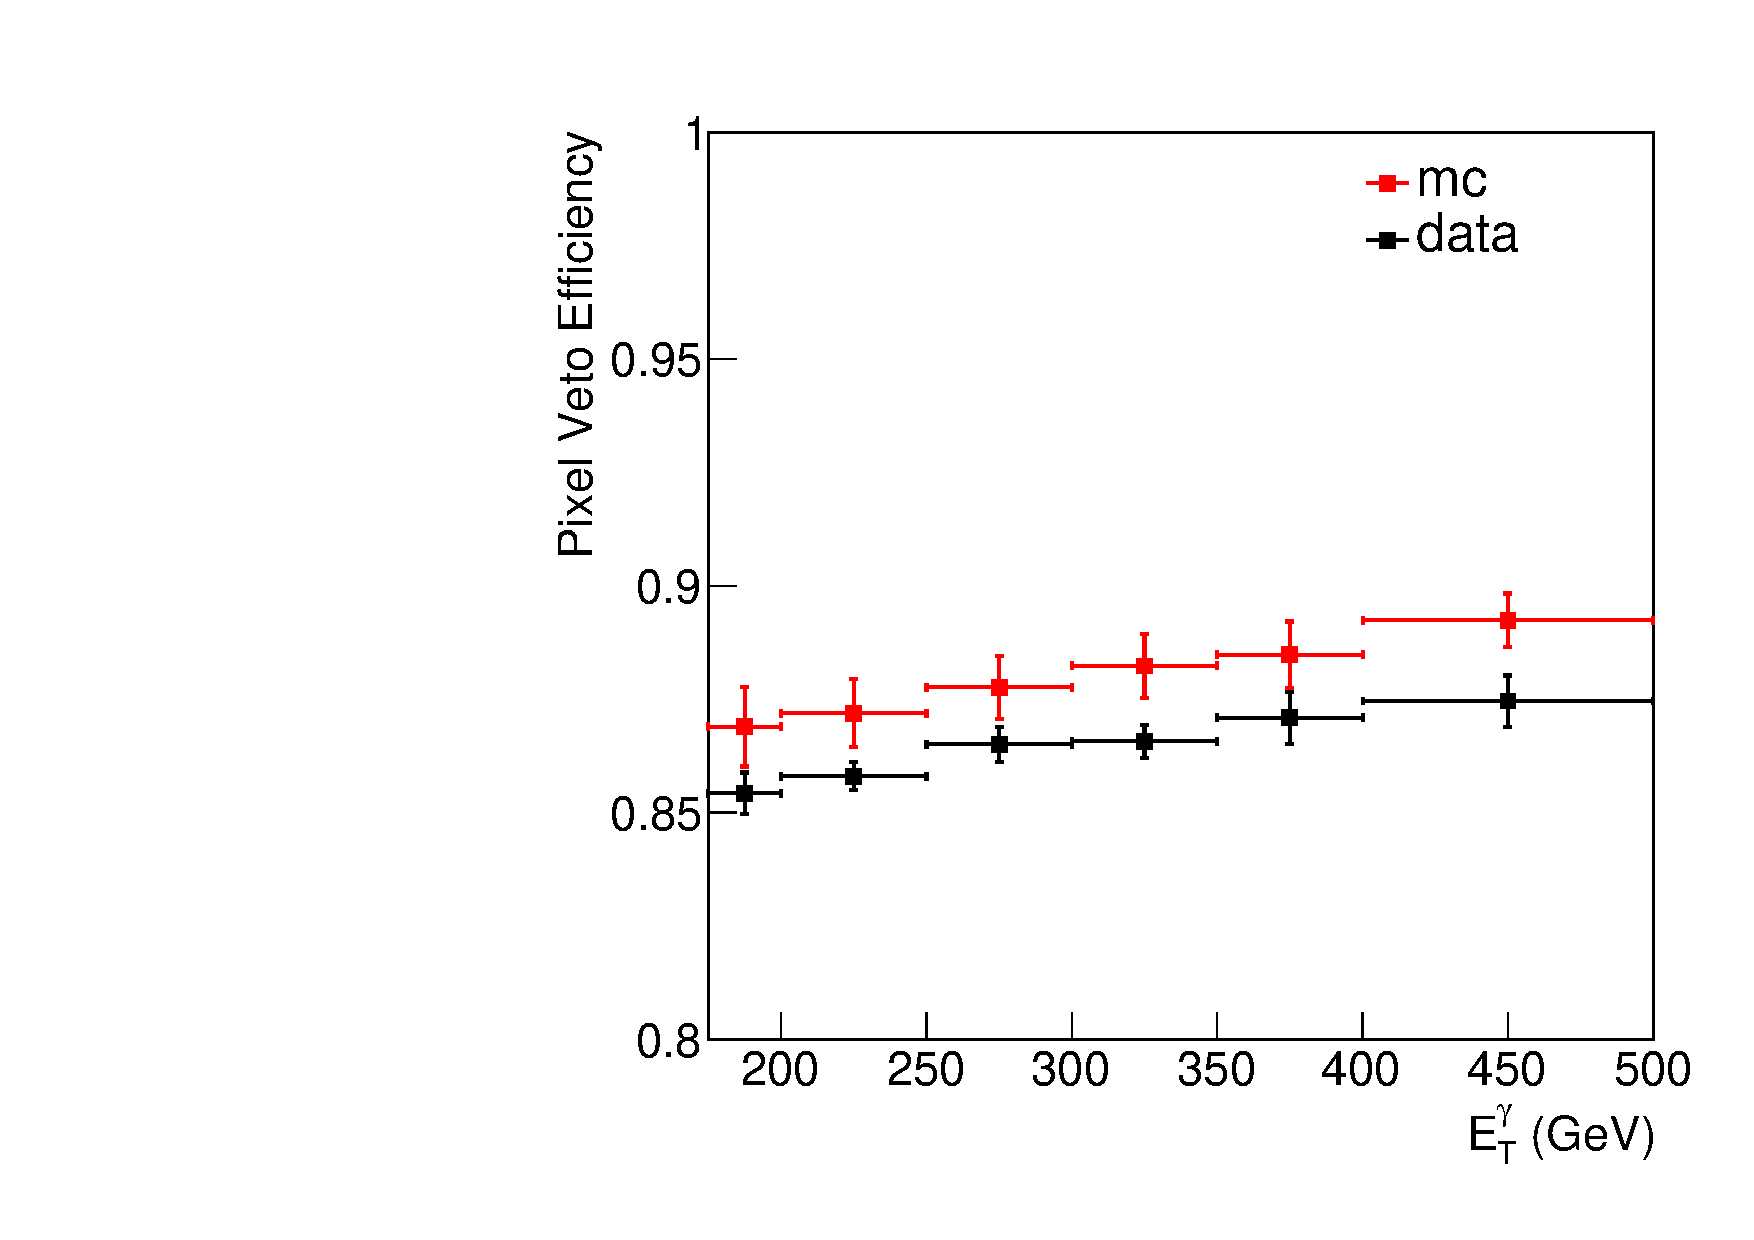
\includegraphics[]{Analysis/Figures/pvsf/efficiency_barrel_medium.pdf}
    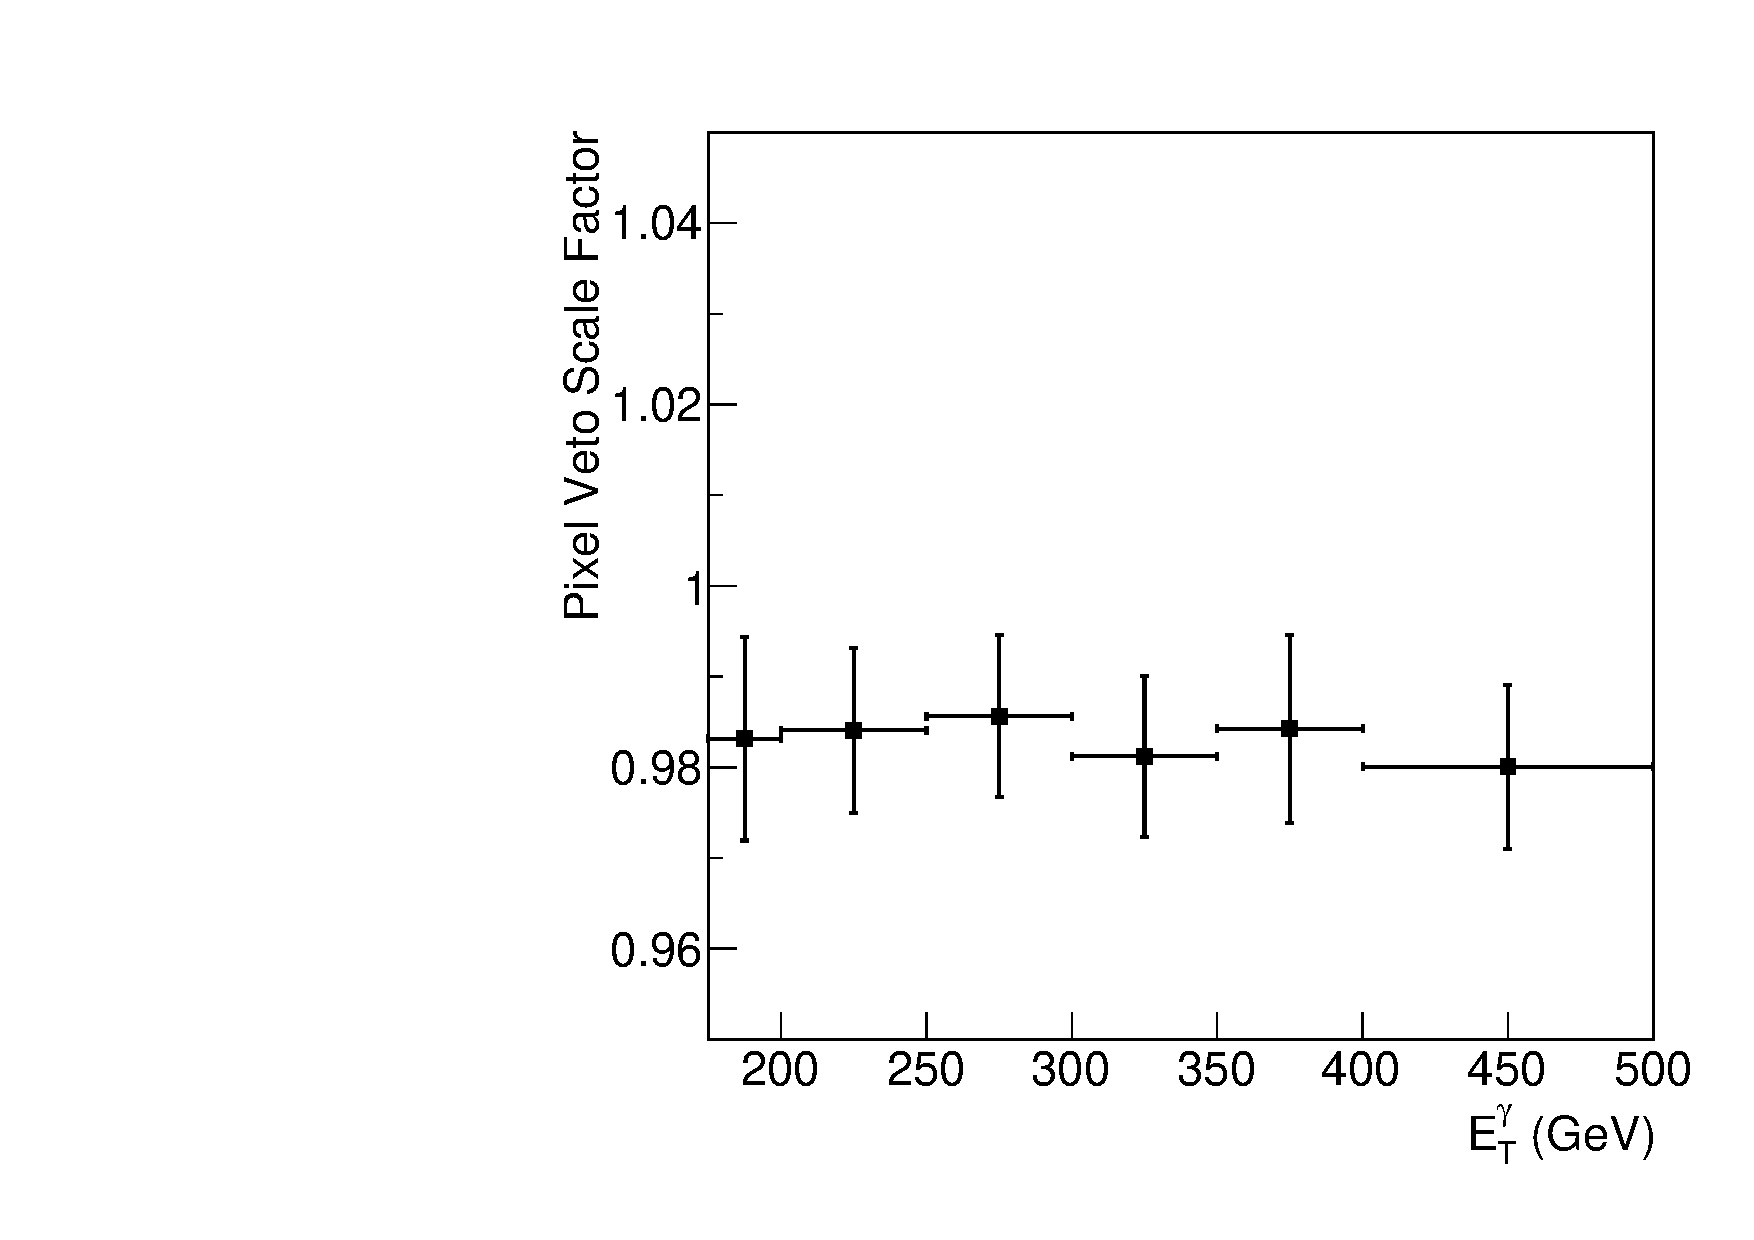
\includegraphics[]{Analysis/Figures/pvsf/scalefactor_barrel_medium.pdf}
  }
  \caption{
    Photon pixel veto efficiencies (left) and correspending scale factor (right) as a function of photon \pt.
  }
  \label{fig:pvsf_results}
\end{figure}
